\documentclass[12pt,a4paper]{report}
\usepackage[utf8]{inputenc}
\usepackage{graphicx}
\usepackage{amsmath}
\usepackage{amssymb}
\usepackage{geometry}
\usepackage{titlesec}
\usepackage{setspace}
\usepackage{caption}
\captionsetup[table]{width=\textwidth}
\captionsetup[figure]{belowskip=-20pt}
\usepackage{fancyhdr}
\usepackage{hyperref}
\usepackage{titletoc}
\usepackage{amsfonts}
\usepackage{longtable}
\usepackage{array}
\usepackage{multirow}
\usepackage{graphicx}
\usepackage{float}
\usepackage[table]{xcolor}
\usepackage[spanish]{babel}
\addto\captionsspanish{\renewcommand{\figurename}{Figura}}
\usepackage{hyperref}
\hypersetup{
    pdfborder={0 0 0}
}
\usepackage[spanish]{babel}
\def\figureautorefname{Figura}
\setcounter{secnumdepth}{3}
\usepackage[style=ieee, backend=biber]{biblatex}
\addbibresource{referencias.bib}
\DefineBibliographyStrings{spanish}{
    url = {Obtenido de:},
    urlseen = {Consultado el},
}
\usepackage{url}
\usepackage{xcolor}
\newcommand{\headlinecolor}{\color{black}}



% Márgenes y espaciado
\geometry{left=3cm, right=2.5cm, top=3cm, bottom=2.5cm}
\newcommand{\hsp}{\hspace{-5pt}}
% Número a la derecha de cada capítulo y espaciado corregido
\titleformat{\chapter}[hang]
  {\vspace{-1cm}
  \headlinecolor\Large\bfseries} % formato
  {\thechapter.\hsp}             % número
  {10pt}                         % separación número - título
  {\Large\bfseries}               % formato del título

% Espaciados capítulos: {izquierda}{antes}{después}
\titlespacing*{\chapter}{0pt}{-8pt}{16pt}

% Espaciados secciones
\titlespacing*{\section}{0pt}{14pt}{8pt}
\titlespacing*{\subsection}{0pt}{10pt}{6pt}

% Para que todo el documento tenga el tipo de letra Arial
\usepackage{fontspec}

% Selecciona Arial como fuente principal
\setmainfont{Arial}

\begin{document}

\renewcommand{\tablename}{Tabla}
\renewcommand{\figurename}{Figura}

\pagenumbering{gobble} % ELIMINA NUMERACION EN PORTADA
\begin{titlepage}
\renewcommand{\baselinestretch}{1.45}\normalsize

\newgeometry{left=3cm,right=3cm,top=3cm,bottom=3cm}
\centering

{\bfseries\fontsize{24}{24}\selectfont ESCUELA POLITÉCNICA NACIONAL\par}\vspace{1.5cm}

{\bfseries\fontsize{16}{20}\selectfont FACULTAD DE INGENIERÍA EN SISTEMAS\par}\vspace{1.5cm}

{\bfseries\fontsize{14}{17}\selectfont OPTIMIZACIÓN DE SISTEMAS DE INFORMACIÓN EN CONTEXTOS EMPRESARIALES\par}\vspace{1cm}

{\bfseries\fontsize{14}{17}\selectfont ANÁLISIS Y SEGMENTACIÓN DE CLIENTES NO REGULADOS DEL SECTOR ELÉCTRICO MEDIANTE ALGORITMOS DE APRENDIZAJE NO SUPERVISADO\par}\vspace{1.5cm}

{\bfseries\fontsize{12}{14}\selectfont TRABAJO DE INTEGRACIÓN CURRICULAR PRESENTADO COMO REQUISITO PARA LA OBTENCIÓN DEL TÍTULO DE INGENIERO EN CIENCIAS DE LA COMPUTACIÓN\par}\vspace{1.5cm}

{\bfseries\fontsize{12}{14}\selectfont ANDRÉS ANTONIO ZAMBRANO ALQUINGA\par}
{\fontsize{12}{14}\selectfont andres.zambrano03@epn.edu.ec\par}\vspace{1cm}

{\bfseries\fontsize{12}{14}\selectfont DIRECTOR: JOSAFÁ DE JESÚS AGUIAR PONTES\par}
{\fontsize{12}{14}\selectfont josafa.aguiar@epn.edu.ec\par}\vspace{1.5cm}

{\bfseries\fontsize{12}{14}\selectfont DMQ, julio 2025\par}
    
\restoregeometry
\end{titlepage}


%% CERTIFICACIONES

\renewcommand{\baselinestretch}{1.25}\normalsize

\pagenumbering{roman} % NUMERACION EN ROMANO
\chapter*{Certificaciones}
\addcontentsline{toc}{chapter}{Certificaciones}

Yo, \textbf{Andrés Zambrano}, declaro que el trabajo de integración curricular aquí descrito es de mi autoría; que no ha sido previamente presentado para ningún grado o calificación profesional; y, que he consultado las referencias bibliográficas que se incluyen en este documento.\\[2cm]
\textbf{NOMBRE\_ESTUDIANTE}\\[1cm]

Certifico que el presente trabajo de integración curricular fue desarrollado por Andrés Zambrano, bajo mi supervisión.\\[2cm]

\textbf{NOMBRE\_DIRECTOR}\\ \textbf{DIRECTOR}



%% DECLARATORIA DE AUTORIA



\chapter*{Declaración de autoría}
\addcontentsline{toc}{chapter}{Declaración de autoría}

A través de la presente declaración, afirmamos que el trabajo de integración curricular aquí descrito, así como el (los) producto(s) resultante(s) del mismo, son públicos y estarán a disposición de la comunidad a través del repositorio institucional de la Escuela Politécnica Nacional; sin embargo, la titularidad de los derechos patrimoniales nos corresponde a los autores que hemos contribuido en el desarrollo del presente trabajo; observando para el efecto las disposiciones establecidas por el órgano competente en propiedad intelectual, la normativa interna y demás normas.\\[2cm]
\textbf{Andrés Zambrano}\\ \textbf{Josafá Aguiar}


% DEDICATORIA


\chapter*{Dedicatoria}
\addcontentsline{toc}{chapter}{Dedicatoria}

A mis padres celestiales, Dios y la santísima Virgen María, en quienes siempre he depositado toda mi fé y confianza a lo largo de toda mi trayectoria académica.\\

\vspace{-2mm}

A mis padres, Verito y Marco, quienes a pesar de todas las dificultades que se presentaron a lo largo del camino, nunca dudaron de mí, y en su lugar, siempre supieron alentarme y darme su apoyo incondicional para seguir adelante, sin lugar a dudas, este, y todos mis logros se los dedico a ustedes. \\

\vspace{-2mm}

A Edita Vélez, mi segunda mamá, quien me cuidó durante toda mi niñez, llenándome siempre de amor, mimos y mucho cariño.\\

\vspace{-2mm}

A mis padrinos, Franklin Vásquez y Silvana Barba, por acogerme con cariño en su hogar durante mis estudios universitarios, de igual manera, a mis primos, Carolina, Dennis y Pamela, quienes más que primos han sido como hermanos para mí.\\

\vspace{-2mm}

A mi primo Jhonny Sánchez, quien ha sido como un hermano para mí, con quien he compartido invaluables momentos durante gran parte de mi niñez. Gracias por ser ese hermano que nunca pude tener, pero que la vida se encargó de darme.\\

\vspace{-2mm}

A la memoria de mis abuelitos, Teresa y Manuel, quienes a pesar de ya no estar físicamente conmigo, sigo sintiendo su amor y protección en cada paso que doy.\\

\vspace{-2mm}

A mis amigos, compañeros de risas, retos e innumerables experiencias, que siempre han estado presentes, tanto en las buenas como en las malas. \\

\vspace{-2mm}

A toda mi familia en general, quienes de manera directa o indirecta han contribuido con su granito de arena para formar la persona que soy hoy en día.\\

\vspace{-2mm}

Finalmente, a mis dos peluditos, Rockie y Merlín, especialmente a mi gordo, Merlín, mi más linda compañía durante mi transición por propedéutico, pasó largas noches de vela a mi lado brindándome de su cálida compañía mientras yo estudiaba.




% AGRADECIMIENTOS




\chapter*{Agradecimientos}
\addcontentsline{toc}{chapter}{Agradecimientos}
Agradezco en primer lugar, a Dios y a la Vírgen María por no desampararme nunca en ninguna etapa de mi vida, por haberme guiado en cada momento, y por empaparme de sabiduría durante toda mi transición por la universidad.\\

\vspace{-2mm}

A mis padres, mis dos grandes tesoros, gracias por creer en mí en todo momento, por demostrarme que con esfuerzo y dedicación todo es posible y, sobre todo, por su amor y apoyo incondicional. Gracias por tanto, gracias por ser mis padres.\\

\vspace{-2mm}

Quiero agradecer de manera muy especial a mi prima Carolina Vásquez por todo lo que ha hecho por mí. Gracias Carito por ser una guía indispensable y un apoyo incondicional en mi vida, eres como una hermana para mí.\\

\vspace{-2mm}

Quiero expresar mi más profundo agradecimiento al Ing. Boris Astudillo por su invaluable orientación, sus sabios consejos y por su constante guía y apoyo a lo largo de mi formación universitaria, en particular durante el desarrollo de mi proyecto de titulación.\\

\vspace{-2mm}

A mi alma máter, la Escuela Politécnica Nacional y a los docentes que contribuyeron a mi formación académica, por brindarme todos los conocimientos y las herramientas necesarias para desarrollarme como profesional.\\

\vspace{-2mm}

Quiero agradecer a todo el equipo de la Empresa Eléctrica Quito, por su apoyo y guía durante el desarrollo de mis prácticas preprofesionales, en especial a los ingenieros e ingenieras Carolina, William, Oscar, Claudia, Isabel y Grace. Agradezco de igual manera al ingeniero Ricardo Dávila por brindarme la confianza y la oportunidad de vivir esta experiencia invaluable para mi desarrollo profesional.\\

\vspace{-2mm}

Finalmente, agradezco a mis amigos Carlos, Alexis, Hernán, Galo, Dilan y los que faltan por nombrar, por hacer que la vida universitaria fuera mucho más llevadera. Gracias por todas las experiencias que compartimos, risas, enojos, tristezas, largas charlas, y sobre todo, la remontada del siglo en sexto semestre.


% ÍNDICE DE CONTENIDOS


\tableofcontents


% RESUMEN


\chapter*{Resumen}

Este Trabajo de Integración Curricular aborda un proyecto de minería de datos enfocado en la implementación de un algoritmo de aprendizaje no supervisado para segmentar clientes en grupos homogéneos a partir de sus curvas características de consumo anual. El objetivo es identificar patrones de consumo energético que permitan una planificación más eficiente y una optimización del uso de la energía en el sector eléctrico.\\

La metodología aplicada es CRISP-DM, con una modificación en su fase final. Dentro de la misma, se han planteado dos procesos claves a seguir: en primer lugar, se desarrolla un proceso ETL orquestado por Apache Airflow, para la consolidación y transformación de los datos mensuales en una curva característica representativa anual por cada cliente, posteriormente, en el proceso de agrupación, se seleccionan y optimizan varios algoritmos para agrupar a los clientes en base a la similitud de sus curvas de consumo.\\

Los resultados de cada algoritmo son evaluados mediante diversas métricas, que cuantifican la calidad de las agrupaciones, con el fin de determinar el algoritmo que ofrece las agrupaciones de mejor calidad. Los resultados de agrupación serán presentados de manera visual y cuantitativa.\\


\textbf{Palabras clave:} minería de datos, segmentación de clientes, curvas de consumo, aprendizaje no supervisado, algoritmos de clustering, planificación energética, proceso ETL, Apache Airflow, CRISP-DM.


% ABSTRACT


\chapter*{Abstract}

This Curriculum Integration Project focuses on a data mining project aimed at implementing an unsupervised learning algorithm to segment clients into homogeneous groups based on their annual characteristic consumption curves. The goal is to identify energy consumption patterns that allow for more efficient planning and optimization of energy use in the electric sector.\\

The methodology applied is CRISP-DM, with a modification in its final phase. Within this framework, two key processes are followed: first, an ETL process orchestrated by Apache Airflow is developed to consolidate and transform monthly data into an annual representative characteristic curve for each client. Then, in the grouping process, several algorithms are selected and optimized to group clients based on the similarity of their consumption curves.\\

The results of each algorithm are evaluated using various metrics that quantify the quality of the groupings, in order to determine which algorithm provides the highest-quality groupings. The grouping results will be presented both visually and quantitatively.\\

\textbf{Keywords:} data mining, customer segmentation, consumption curves, unsupervised learning, clustering algorithms, energy planning, ETL process, Apache Airflow, CRISP-DM.

\newpage
\pagenumbering{arabic} % NUMERACION NORMAL

% INTRODUCCIÓN

\chapter{DESCRIPCIÓN DEL COMPONENTE DESARROLLADO}


En el contexto actual de las empresas proveedoras de energía, como la Empresa Eléctrica Quito (EEQ), la eficiente gestión energética es uno de los principales desafíos a enfrentar. Múltiples factores como la diversificación en los hábitos de consumo y variablidad de la demanda dificultan la planificación y diseño de estrategias eficientes que permitan responder de manera adecuada. Los métodos tradicionales de análisis, que se basan en promedios o clasificaciones rígidas resultan insuficientes para capturar dicha complejidad en los patrones de consumo de los clientes, dificultando el diseño de una planificación energética eficiente.\\

Con el fin de optimizar la distribución de recursos en áreas como la gestión tarifaria y la distribución eléctrica, es fundamental analizar los patrones de consumo. La identificación de estos patrones en el comportamiento energético de los clientes brinda la posibilidad de definir segmentos con características similares, permitiendo a las compañías proveedoras de energía establecer una base más firme para la toma de decisiones.\\

Ante esta problemática, se ha desarrollado un componente orientado a la segmentación inteligente de clientes, implementando un proyecto de minería de datos que propone un enfoque basado en técnicas de aprendizaje no supervisado con el fin de generar grupos homogéneos en función de la forma de su curva característica anual de consumo energético. El objetivo principal es identificar patrones de consumo que permitan una planificación más eficiente y optimización del uso de la energía en el sector eléctrico.\\

Bajo este contexto, el desarrollo del componente es realizado bajo la metodología CRISP-DM, con una ligera modificación en su fase final. Mientras que en la metodología original la fase final se centra en la implementación y despliegue del modelo, en este caso, el objetivo final es, entre todas las agrupaciones dadas por los diferentes algoritmos, escoger aquella que tenga la mejor calidad y homogeneidad, basándose en métricas de evaluación. Esta modificación de la fase final es posible debido a que CRISP-DM es sumamente flexible, y permite personalizar sus fases en función de los objetivos del proyecto.\\ 

Dentro del flujo de trabajo estructurado que propone la metodología CRISP-DM, se han definido dos procesos claves: en primer lugar, se lleva a cabo un proceso de Extracción, Transformación y Carga (ETL), orquestado por Apache Airflow, para normalizar y consolidar los datos de consumo mensual de cada cliente en una curva representativa anual.\\

Posteriormente, se desarrolla el proceso de agrupación, donde se determina el número óptimo de grupos de clientes a través de un análisis conjunto con las partes interesadas y el uso de métodos de validación como el método del codo. Se implementan y optimizan diferentes algoritmos de clustering, como KMeans, GaussianMixture, Birch y Spectral Clustering, para segmentar a los clientes en base a la similitud de sus curvas de consumo. Finalmente, se evalúan los resultados de cada algoritmo utilizando diversas métricas, como Silhouette Score, SSE, Davies-Bouldin Index y Calinski-Harabasz Index, para seleccionar el algoritmo que ofrezca las mejores agrupaciones. Los resultados obtenidos serán presentados tanto de manera visual como cuantitativa, permitiendo una interpretación clara y precisa de las agrupaciones logradas.

\section{Objetivo general}

Evaluar e implementar modelos de aprendizaje no supervisado para la segmentación de clientes no regulados del sector eléctrico utilizando curvas de carga para la obtención de agrupaciones homogéneas.

\section{Objetivos específicos}

\begin{enumerate}
    \item Levantar requerimientos para la obtención y procesamiento de los datos de consumo energético de los clientes no regulados, transformándolos en curvas de carga representativas para su almacenamiento en una base de datos.
    \item Realizar una revisión literaria de los algoritmos de agrupamiento más relevantes, identificando su funcionamiento, principios y parámetros claves para su correcta optimización e implementación en la segmentación de clientes del sector eléctrico.
    \item Implementar una metodología de análisis de datos para la ejecución del proceso sistemático encargado de guiar las diferentes fases.
    \item Aplicar los algoritmos de clustering, utilizando métodos de validación para definir el número óptimo de agrupaciones.
    \item Evaluar y presentar los resultados generados por cada algoritmo, utilizando visualizaciones detalladas de las curvas de carga agrupadas.
\end{enumerate}

\section{Alcance}

Como se mencionó en la descripción del componente, el presente trabajo está enmarcado en el análisis y segmentación de clientes no regulados del sector eléctrico, a partir de la construcción de sus curvas de carga características y la posterior aplicación de algoritmos de aprendizaje no supervisado con el fin de identificar patrones de consumo energético. El alcance de este trabajo está definido bajo las siguientes consideraciones:

\begin{enumerate}
    \item Se ha adoptado la metodología CRISP-DM como marco de referencia, con una adaptación en su fase final. Dicha fase implica originalmente el despliegue del modelo en un entorno productivo, pero en este trabajo va a enfocarse en la evaluación comparativa de los resultados obtenidos con diferentes algoritmos de clustering, donde se presentarán métricas cuantitativas así como visualizaciones interpretativas de las agrupaciones.
    \item Se llevará a cabo un proceso ETL, el cual obtiene, integra, limpia y normaliza los registros históricos de consumo energético que se tienen de cada cliente, con la finalidad de generar curvas de carga que representen el comportamiento energético de cada cliente. Este proceso contempla la interpolación de valores nulos, la exclusión de días no laborales, corrección de formatos inconsistentes y la normalización mediante técnicas de escalamiento.
    \item Se realizará la optimización e implementación de varios algoritmos de clustering (KMeans, GaussianMixture, Birch y Spectral Clustering), los cuales serán seleccionados en función de su relevancia en la literatura y su aplicabilidad en el análisis de análisis de curvas de carga. Para determinar el número óptimo de agrupaciones se hará uso de métodos de validación como el método del codo. Por otro lado, para la optimización de estos algoritmos se utilizará la correlación intra-cluster, esta métrica es la más adecuada pues captura de mejor manera la similitud en forma de las curvas agrupadas.
    \item Los resultados incluirán la curva de carga representativa de cada cliente, la curva de carga correspondiente al día de máxima demanda, archivos .csv con las coordenadas de dichas curvas. Asimismo, se presentarán resultados visuales de los clústeres y una tabla comparativa con métricas que cuantifican la calidad de las agrupaciones generadas por cada algoritmo.
    \item Para el desarrollo del presente componente se ha contemplado Python como lenguaje de programación de alto nivel, Visual Studio Code como entorno de desarrollo integrado, bibliotecas especializadas en análisis de datos y machine learning (pandas, scikit-learn, numpy, matplotlib, entre otras), así como herramientas de orquestación, en este caso Apache Airflow sobre Docker, para la automatización del proceso ETL.
\end{enumerate}

Por lo anterior expuesto el alcance del componente se limita a la construcción, aplicación y evaluación de modelos de clustering basados en la similitud de curvas de carga, sin abordar fases posteriores como despliegues productivos en entornos de la empresa distribuidora de energía.

% MARCO TEÓRICO

\section{Marco Teórico}

Para comprender este trabajo y su contexto, es de gran importancia tener bases sólidas sobre los principios subyacentes que sustentan el análisis y agrupación de los clientes en función de su curva de carga. Los apartados siguientes explicarán conceptos claves dentro del desarrollo del presente componente.

\subsection{Sobre el sector eléctrico}\\
\begin{enumerate}
\item{\textbf{Clientes no regulados}}\\
Los clientes no regulados en el sector eléctrico son aquellos cuya facturación por el suministro de energía se rige estrictamente por un contrato a término, el cual es realizado entre la empresa que suministra la energía y la empresa que recibe dicha energía. Los contratos mencionados anteriormente son bilaterales\cite{conelec2012}.

Debido a la naturaleza de los contratos que se suscriben con este tipo de clientes, los patrones de consumo de energía que poseen son bastantes variados respecto a los clientes regulados \cite{conelec2012}.


\item{\textbf{Curvas típicas (curva de carga)}}\\
Una curva de carga o también llamada curva típica es un registro gráfico que indica la demanda eléctrica que ha tenido un cliente en cada instante durante un intervalo de tiempo determinado\cite{curva_carga_1}.

Estas curvas de carga reflejan el patrón de consumo cotidiano que poseen los clientes, dicho patrón está directamente relacionado con las máquinas o aparatos que utilizan, así como la energía que consumen durante sus actividades\cite{curva_carga_2}.

\clearpage
\item{\textbf{Segmentación de clientes}}\\
Debido a la naturaleza de los clientes no regulados y, agregando el hecho de que en su mayoría son grandes clientes, segmentarlos en grupos homogéneos permite optimizar la gestión de la demanda y mejorar la planificación del suministro eléctrico. Al agrupar clientes con patrones de consumo similares, es posible diseñar estrategias más eficientes para la contratación de energía, desarrollar y optimizar modelos tarifarios y, mejorar la predicción de la demanda a futuro \cite{curva_carga_1}. Además, esta segmentación ayuda a evitar el sobredimensionamiento o subdimensionamiento de la capacidad de generación y distribución, garantizando un uso más eficiente de los recursos y optimizando los costos operativos.
\end{enumerate}

\subsection{Minería de datos}
Según \cite{datamining-1}, la minería de datos corresponde a un proceso que consiste en la extracción de información relevante a partir de un gran conjunto de datos, con el fin de encontrar patrones interesantes que sean de utilidad, los cuales de otro modo habrían pasado desapercibidos. De la misma manera, métodos tradicionales de análisis de datos son combinados con algoritmos capaces de manejar grandes volúmenes de datos \cite{datamining-2}. Entre sus principales funciones se destacan \cite{datamining-2}:
\begin{enumerate}
\item \textbf{Caracterización/Discriminación:} Sintetizar y explicar clases o conceptos.
\item \textbf{Patrones frecuentes y asociaciones:} Reconocer relaciones que se repiten en el conjunto de datos.
\item \textbf{Clasificación y regresión:} Elaborar modelos para predecir clases o valores numéricos.
\item \textbf{Agrupación:} Generar etiquetas a partir de datos sin clasificar, optimizando la similitud interior.
\item \textbf{Detección de valores atípicos:} Reconocer datos que no se ajustan a un patrón general.
\end{enumerate}

En el contexto de la minería de datos, diversas metodologías han sido propuestas con el fin de dotar de estructura y sistematicidad a este proceso. Estas metodologías proveen fases bien definidas con el fin de asegurar la coherencia entre los objetivos del proyecto y los resultados. A continuación se detallan las tres metodologías más reconocidas en la literatura:

\begin{enumerate}
    \item \textbf{KDD (Knowledge Discovery in Databases)}\\
    KDD fue el primer modelo en recibir aprobación por parte de la comunidad científica para dirigir proyectos cuyo propósito es la obtención de conocimiento a partir de grandes cantidades de datos \cite{moine2011estudio}. Esta metodología plantea un proceso iterativo que incluye la selección de datos, preprocesamiento, transformación, la implementación de algoritmos y el análisis de patrones. Entre sus contribuciones relevantes destaca la distinción de la minería de datos como una fase que forma parte de un proceso más amplio \cite{plotnikova2020adaptations}. A diferencia de otras metodologías posteriores, a KDD se le atribuye un enfoque fundamentalmente conceptual, debido a que establece de manera generalizada cada fase del descubrimiento de conocimiento, sin profundizarlas \cite{moine2011estudio}. KDD es visto como un punto de inicio para la sistematización de la minería de datos debido an esta característica, ya que proporcionó una base para el desarrollo de modelos más integrales que surgieron en años siguientes \cite{moine2011estudio}.
    \item \textbf{CRISP-DM (Cross-Industry Standard Process for Data Mining)}\\
    La metodología CRISP-DM, establecida en el año 2000, ha logrado consolidarse como la más utilizada para proyectos vinculados con la minería de datos \cite{moine2011estudio}. Comprende seis etapas: entendimiento del negocio, entendimiento de los datos, preparación de los datos, modelado, evaluación y despliegue. En este modelo se detalla claramente las tareas y actividades que se deben llevar a cabo en cada fase, lo que permite establecer una conexión entre los objetivos estratégicos y el análisis técnico, es gracias a este equilibrio que CRISP-DM se posiciona como un marco idóneo para proyectos académicos e industriales \cite{plotnikova2020adaptations}. Esta metodología admite retrocesos dentro de su flujo de trabajo, también permite realizar cambios en sus fases en función de los objetivos del proyecto, lo que refuerza su naturaleza iterativa y la hace muy flexible \cite{plotnikova2020adaptations}.
    \item \textbf{SEMMA (Sample, Explore, Modify, Model, Assess)}\\
    SEMMA es un modelo desarrollado por el instituto SAS, establece una guía metodológica que estructura un proceso en cinco fases: muestreo, exploración, modificación, modelado y evaluación \cite{moine2011estudio}. Cada fase está enfocada en los aspectos técnicos del tratamiento de datos y en la aplicación de algoritmos. A diferencia de CRISP-DM, SEMMA no contempla las fases de comprensión del negocio o despliegue, situándola como una metodología muy útil en la ejecución de tareas relativas al análisis de datos, pero ineficaz para tareas donde los objetivos de la organización son clave \cite{plotnikova2020adaptations}. Su utilidad se encuentra en proyectos en los que la experimentación y el modelado son más importantes que integrar el conocimiento adquirido dentro de los procesos comerciales \cite{plotnikova2020adaptations}.
\end{enumerate}

\clearpage
\subsection{Proceso ETL}
El proceso ETL, es una técnica crucial que sirve para obtener, organizar y usar los datos apropiadamente según el fin requerido, se enfoca principalmente en la unión de datos provenientes de diversas fuentes, así como de su evaluación y limpieza \cite{singu2022etl}. Tal y como sus siglas indican, este proceso involucra tres fases descritas a continuación:

\begin{enumerate}
    \item \textbf{Extracción}: Este paso es el responsable de extraer el conjunto requerido de datos de una o más fuentes, donde cada fuente  tiene sus propias características, por lo cual, se debe tener conocimiento sobre como acceder a dichas fuentes, comprender la estructura de las mismas y saber como manejar cada fuente de acuerdo a su naturaleza \cite{elsappagh2011proposed}. Este proceso termina cuando todo el conjunto de datos es consolidado en un solo repositorio \cite{elsappagh2011proposed}.
    \item \textbf{Transformación}: Esta segunda fase consiste en procesar los datos extraídos para que sean consistentes, limpios e integrables dentro del repositorio. Se realizan diversas tareas como reestructurar la información, convertir formatos, limpiar los datos, integrar múltiples fuentes, tratamiento de valores nulos, entre otros \cite{inmon2002building}. El objetivo es asegurar que la información esté depurada y en condiciones para su carga en el repositorio final \cite{inmon2002building}.
    \item \textbf{Carga}: Es la última fase, aquí los datos son almacenados en un repositorio final o en una base de datos para su posterior análisis \cite{gour2010improve}.
\end{enumerate}

\subsection{Aprendizaje no supervisado}
El aprendizaje no supervisado es un tipo de algoritmo de aprendizaje automático, utiliza únicamente datos sin etiquetar, y es usado sobre estos con el objetivo de descubrir patrones o agrupar datos que posiblemente comparten características similares entre sí \cite{Wang2022_unsupervised_machine_learning_urban_studies}. En este contexto, es pertinente destacar algunos elementos clave que permitirán una mejor comprensión, tales como:

\begin{enumerate}
\item\textbf{Clustering}\\
Es una de las categorías del aprendizaje no supervisado, la más consolidada en la actualidad, su objetivo es la identificación de subgrupos dentro de un conjunto extenso de datos no procesados, estos subgrupos son encontrados mediante la diferenciación de características \cite{Wang2022_unsupervised_machine_learning_urban_studies}.
\item\textbf{Número de agrupaciones}\\
Un problema muy común al utilizar algoritmos de aprendizaje no supervisado es elegir el número de agrupaciones deseadas \cite{CoraggioCoretto2021_clusters_quadratic_discriminant_score}, esta elección es muy importante debido a que puede alterar la calidad de las agrupaciones finales dadas por los algoritmos. Como se menciona en \cite{Lezhnina2022_latent_class_cluster_analysis}, esta elección puede ser totalmente subjetiva, y en la mayoría de los casos el números de agrupaciones es seleccionado en función de criterios preestablecidos, sin embargo, existen técnicas como el método del codo que ayudan a validar el número de agrupaciones y que pueden ayudar en la selección de este critero.
\item\textbf{Método del codo}\\
Es la forma más habitual de elegir o validar el número de clústeres, este método consiste en ajustar varios modelos K-means para un rango específico de agrupaciones, normalmente desde 1 hasta un número arbitrario máximo, posteriormente se traza un gráfico que contiene el valor total de la suma de los cuadrados por cada número de clústeres frente a ese respectivo número de clústeres \cite{Friedman2017_survey_R_packages_cluster_analysis}. El objetivo es encontrar aquel valor de número de clústeres donde la gráfica muestra un 'codo' y elegir dicho valor que probablemente nos ofrezca grupos bien separados \cite{Friedman2017_survey_R_packages_cluster_analysis}.

\item\textbf{Algoritmos de clustering}\\
Los algoritmos de clustering son una parte fundamental del aprendizaje no supervisado, pues facilitan el descubrimiento de estructuras y patrones ocultos dentro de un conjunto de datos sin etiquetar \cite{wani2024comprehensive}.

A continuación se describirán los algoritmos de clustering que van a ser utilizados para el desarrollo del presente componente: 

\begin{enumerate}
    \item \textbf{K-Means} \\
    Algoritmo de clustering basado en centroides que organiza $n$ puntos de datos en $k$ clústeres según la proximidad a centroides representativos \cite{wani2024comprehensive}. 
    Cada centroide corresponde a la media de su clúster y el objetivo es minimizar la suma de las distancias al cuadrado entre cada punto y su centroide \cite{wani2024comprehensive}, se puede formular matemáticamente como:
    
    {\setlength{\abovedisplayskip}{-8pt}
    \setlength{\belowdisplayskip}{8pt}\begin{equation}
        J = \sum_{i=1}^{k} \sum_{\mathbf{x}\in S_i} \|\mathbf{x} - \mu_i\|^2 
        \quad \text{con} \quad 
        \mu_i = \frac{1}{|S_i|}\sum_{\mathbf{x}\in S_i} \mathbf{x} 
        \quad \text{y} \quad 
        i = \arg\min_j \|\mathbf{x} - \mu_j\|^2
    \end{equation}}

    \item \textbf{Gaussian Mixture Models (GMM)} \\
    Modelo que asume que los datos provienen de una mezcla de Gaussianas, cada una definida por su media y covarianza \cite{wani2024comprehensive}. 
    Este enfoque permite representar estructuras multimodales donde K-means falla. 
    Los parámetros se estiman con el algoritmo EM, que ajusta iterativamente medias, covarianzas y pesos para representar mejor los datos \cite{wani2024comprehensive}. Matemáticamente, el modelo es expresado como:
    
    {\setlength{\abovedisplayskip}{-8pt}
    \setlength{\belowdisplayskip}{8pt}\begin{equation}
        p(x) = \sum_{j=1}^{k} \pi_j N(x|\mu_j, \Sigma_j), 
        \qquad 
        w_{ij} = \frac{\pi_j N(x_i|\mu_j, \Sigma_j)}
        {\sum_{l=1}^{k} \pi_l N(x_i|\mu_l, \Sigma_l)}
    \end{equation}}
    
    mientras que las actualizaciones de los parámetros en cada iteración están dadas por:

    {\setlength{\abovedisplayskip}{-2pt}
    \setlength{\belowdisplayskip}{8pt}\begin{equation}
        \pi_j = \frac{1}{n}\sum_{i=1}^{n} w_{ij}, 
        \quad 
        \mu_j = \frac{\sum_{i=1}^{n} w_{ij} x_i}{\sum_{i=1}^{n} w_{ij}}, 
        \quad 
        \Sigma_j = \frac{\sum_{i=1}^{n} w_{ij}(x_i-\mu_j)(x_i-\mu_j)^{T}}
        {\sum_{i=1}^{n} w_{ij}}
    \end{equation}}
        

    \item \textbf{Spectral Clustering} \\
    Algoritmo de clustering basado en grafos, transforma los datos en una red donde los nodos representan puntos de datos y las aristas sus similitudes, a partir de esto construye la matriz Laplaciana, cuyos autovectores permiten identificar estructuras dentro del grafo y formar clústeres con alta cohesión interna \cite{wani2024comprehensive}. El objetivo es minimizar la siguiente función:
    
    {\setlength{\abovedisplayskip}{-20pt}
    \setlength{\belowdisplayskip}{8pt}\begin{equation}
        \min \; \text{Tr}(H^{T} L H) \quad \text{sujeto a} \quad H^{T}H = I
    \end{equation}}
        

    \item \textbf{BIRCH} \\
    Es un algoritmo de clustering de tipo jerárquico, está diseñado para trabajar con grandes volúmenes de datos, resumiendo toda la información de los mismos en una sola estructura jerárquica que tiene el nombre de CF-Tree, donde cada clúster es representado como una Clustering Feature (CF) \cite{fontanini2018birch}, la cual está definida por:

    {\setlength{\abovedisplayskip}{1pt}
    \setlength{\belowdisplayskip}{8pt}\begin{equation}
    CF = (N, LS, SS)
    \end{equation}}
    
    donde $N$ es el número de puntos, $LS$ la suma lineal y $SS$ la suma de los cuadrados de los datos. El umbral de radio $T$ se determina mediante un problema de optimización, definido como:

    {\setlength{\abovedisplayskip}{1pt}
    \setlength{\belowdisplayskip}{3pt}\begin{equation}
    \min_T \; g(W_k(T), B_k(T))
    \end{equation}}
    
    donde $W_k$ mide compacidad intra-clúster y $B_k$ separación inter-clúster \cite{fontanini2018birch}.

\end{enumerate}

\clearpage
\item\textbf{Hiperparametrización de algoritmos}\\
Técnica que consiste en ajustar los parámetros que controlan el comportamiento de los algoritmos de clustering, estos parámetros influyen en la calidad de las agrupaciones finales, el objetivo es encontrar aquella combinación de parámetros que ofrezca los mejores resultados en cada algoritmo \cite{pathak2024randomized}. 

\item\textbf{Métricas de evaluación de agrupaciones}\\
Son medidas de calidad que sirven para dar validación a los clústeres obtenidos por los algoritmos, estas métricas se basan en la premisa de 'Maximizar la similitud dentro de cada clúster y minimizar la similitud entre los diferentes clústeres', el objetivo es lograr clústeres compactos y lo más separados posibles entre sí \cite{heras2023tfg}.
\end{enumerate}

\vspace{-0.45cm}

\subsection{Herramientas utilizadas}
Para el desarrollo del componente se han considerado varias herramientas que facilitan las etapas de procesamiento, almacenamiento, análisis de los datos, e implementación de los modelos de clustering, la Tabla \ref{tab:herramientas} los detalla:

\vspace{-0.025cm}

%\begin{footnotesize}
\begin{longtable}{|p{2.5cm}|p{12.3cm}|}
\caption{{{Herramientas utilizadas para el desarrollo del componente}} \label{tab:herramientas}} \\
\hline
\textbf{Herramienta} & \textbf{Descripción de la herramienta} \\
\hline
\endfirsthead

\hline
\textbf{Herramienta} & \textbf{Descripción de la herramienta} \\
\hline
\endhead

\hline
\endfoot

\hline
\endlastfoot

Airflow 2.10.5 & Apache Airflow es una plataforma de código abierto que permite el desarrollo, programación y supervisión flujos de trabajo, utiliza Python, lo que le permite conectarse con diversas tecnologías \cite{airflow_docs}. \\ \hline

Docker 4.43.1 & Docker es una plataforma abierta utilizada para el desarrollo, envío y ejecución de aplicaciones, permite empaquetar y ejecutar aplicaciones en un entorno aislado denominado contenedor \cite{docker_docs}. \\ \hline

Python 3.13 & Python es un lenguaje de programación de alto nivel con naturaleza interpretada, maneja estructuras de datos con un alto nivel de eficiencia y ofrece una sintaxis simple, razones por las cuales es ampliamente utilizado en campos como desarrollo web, ciencia de datos, automatización, entre otros \cite{python_docs}. \\ \hline

Visual Studio Code 1.101.2 & Visual Studio Code es un editor de código fuente que contiene herramientas de depuración, control de versiones y extensiones para varios lenguajes. Ofrece varias características que permiten desarrollar código eficientemente \cite{vscode_docs}.\\ \hline

MongoDB Atlas 8.0.13 & Es una base de datos no relacional administrada en nube, basada en documentos, y que brinda una gran escalabilidad y flexibilidad, además de un modelo avanzado de consultas e indexación \cite{mongodb_docs}.\\
\hline

\end{longtable}
%\end{footnotesize}

% METODOLOGÍA






\chapter{Metodología}
\vspace{-0.5cm}
\section{Caso de estudio}
Unos de los grandes desafíos que enfrenta la Empresa Eléctrica Quito (EEQ) es la administracion eficiente de la demanda de sus clientes, especialmente la de aquel segmento que no está regulado, este grupo de clientes es estratégico debido a su representativo nivel de consumo y a la variablidad de sus patrones de carga. Estos usuarios, no están incluidos en un esquema tarifario regulado, por lo cual exhiben una gran diversidad en sus curvas de demanda. Esto obstaculiza enormemente la planificación energética y el diseño de estrategias destinadas a asegurar eficiencia y fiabilidad en el sistema eléctrico.\\

Los métodos tradicionales que han sido utilizado en la EEQ con el fin de examinar el comportamiento de la demanda (basados principalmente en clasificaciones rígidas o en el cálculo de promedios), han demostrado importantes limitaciones al no conseguir captar la complejidad de los patrones de consumo. En investigaciones anteriores realizadas por Gerencia de Planificación, se ha confirmado esta circunstancia. Los estudios mostraron que el comportamiento energético está directamente relacionado con la actividad económica del cliente no regulado y a su curva de carga característica, lo cual hace inviable que un único criterio generalizado represente apropiadamente a todo este conjunto.

\section{Brainstorming}
La lluvia de ideas, también conocida como brainstorming, es un método que se emplea en el campo de la ingeniería de requisitos y la investigación para recopilar información de manera colaborativa. Esto facilita determinar necesidades, cuestiones problemáticas y posibles perspectivas de solución deurante las etapas iniciales de un proyecto. Su valor metodológico radica en su capacidad de permitir reunir un conjunto extenso de percepciones, las cuales pueden ser organizadas y analizadas con más rigor posteriormente, convirtiéndose así en un insumo fundamental para determinación del enfoque metodológico \cite{Weichbroth2016}.\\

En relación con el desarrollo del presente componente, esta técnica se utilizó como método para recopilar información en reuniones con el equipo encargado del departamento de planificación de la demanda. Los métodos de análisis tradicionales, la disparidad de los perfiles de carga y la necesidad de contar con un mecanismo de segmentación que facilite la agrupar a los clientes según su comportamiento energético fueron determinados mediante este proceso.\\

La relevancia del uso de brainstorming en este caso de estudio se explica por el hecho de que, siendo un problema técnico y organizacional complejo, fue imprescindible obtener directamente la experiencia y la sabiduría del personal de la compañía. De este modo, esta técnica hizo posible determinar las necesidades y los problemas más importantes vinculados al estudio del comportamiento energético de los clientes no regulados, lo cual permitió establecer un punto de partida claro para el desarrollo del proyecto.

\section{CRISP-DM}\\
El desarrollo del presente componente se sustenta en CRISP-DM, cuyas siglas corresponden a Cross-Industry Standard Process for Data Mining, metodología que es ampliamente reconocida por su aplicabilidad en proyectos de minería de datos y por brindar un enfoque sistemático y estructurado.\\

La elección de esta metodología se basa en la necesidad de guiar de manera ordenada el análisis del consumo energético de los clientes no regulados del sector eléctrico, y esta opción es la que más se acopla debido a que nos permite avanzar desde la comprensión del problema hasta la obtención de resultados comparables. Además, la metodología CRISP-DM brinda la flexibilidad necesaria para realizar ajustes en sus fases en función de los objetivos que se quieran cumplir, esta característica fue clave para su elección, pues en el presente componente la fase final no contemplará un despliegue productivo como tal, sino una evaluación comparativa de la calidad de agrupaciones obtenidas por cada algoritmo.\\

La validez del uso de CRISP-DM para el desarrollo del presente componente es respaldada por su probado éxito en estudios anteriores similares a este. Sarnovsky y Bednár aplicaron en \cite{sarnovsky2025} esta metodología para realizar clustering de clientes de una empresa distribuidora de energía, donde estos fueron agrupados en función de sus curvas de carga anuales. De manera similar, Otieno adoptó CRISP-DM en \cite{otieno2021} como base para desarrollar diversos análisis de patrones de consumo en una empresa distribuidora de energía. Incluso en otros sectores, como el de software, investigaciones como la presentada en \cite{ijiepr2021} emplean CRISP-DM para estructurar procesos de clustering de clientes basados en técnicas de minería de datos. Estos antecedentes proporcionan una evidencia sólida y específica que valida la elección de CRISP-DM como metodología para el desarrollo del presente componente.\\

CRISP-DM es un método probado utilizado para orientar proyectos de minería de datos. Ofrece una serie de fases que resúmen el ciclo vital de minería de datos, a la vez que incluye descripciones y tareas necesarias en cada fase, ayudando a estructurar un flujo de trabajo ordenado cuya secuencia no es estricta, donde se puede avanzar y retroceder entre fases de ser necesario \cite{crisp-dm1}.\\

El modelo CRISP-DM es sumamente flexible, y sus fases pueden ser personalizadas en función de los objetivos del proyecto, pudiendo crear un modelo de minería de datos que se adapte a necesidades concretas \cite{crisp-dm1}. CRISP-DM contiene un total de seis fases, tal y como se describe en \cite{crisp-dm2}:

\begin{enumerate}
    \item \textbf{Comprensión del negocio:} Esta fase inicial se enfoca en analizar y comprender tanto los objetivos como los requerimientos del proyecto desde la perspectiva del negocio. Posteriormente todo este conocimiento es plasmado en un proyecto de minería de datos enfocado en alcanzar los objetivos.
    
    \item \textbf{Comprensión de los datos:} La fase de comprensión de datos tiene como principal objetivo la 'familiarización' con los datos. Para lograr esto se realiza una recolección inicial de los datos y se procede a realizar un pequeño análisis exploratorio de los datos con el fin de comprender los datos que se tienen e identificar problemas con la calidad de los mismos.
    
    \item \textbf{Preparación de los datos:} Esta fase es crucial en CRISP-DM, debido a que abarca todas las actividades requeridas hasta la construcción final del conjunto de datos, los cuales servirán posteriormente para la fase de modelado. Esta fase incluye tareas como la limpieza, transformación y normalización de los datos, con el fin de asegurar la calidad de estos.
    
    \item \textbf{Modelado:} Varias herramientas de modelamiento son seleccionadas con el fin de ser aplicadas sobre nuestro conjunto de datos preparados. Los parámetros de dichas herramientas deben ser calibrados hasta obtener los valores óptimos que ofrezcan los mejores resultados.
    
    \item \textbf{Evaluación:} En esta penúltima fase del proyecto, ya se tiene construido uno o varios modelos que aparentemente ofrecen resultados de calidad. Antes de proceder a la fase del despliegue, se realiza una evaluación del modelo, revisando cada paso ejecutado hasta la construcción final del mismo con el fin de determinar si existe algún objetivo que no haya sido abordado lo suficiente.
    
    \item \textbf{Despliegue:} La construcción del modelo no es el final del proyecto. En función de los requerimientos, la fase de despliegue puede ser tan simple como la generación de un reporte o tan complejo como su respectiva implementación en otros proyectos de minería de datos.
    
\end{enumerate}

Es importante recalcar que, en el desarrollo del presente componente, la fase número seis de CRISP-DM correspondiente al despliegue fue modificada en función de los objetivos específicos del proyecto. En este caso, a diferencia de la metodología original, que incluye en esta fase la implementación del modelo en un entorno productivo, en este caso, esta fase tendrá un enfoque comparativo de los resultados obtenidos con los distintos algoritmos de clustering. Para ello, las agrupaciones fueron analizadas mediante el uso de métricas de evaluación que permiten cuantificar la calidad de los clústeres, con la finalidad de elegir aquellos resultados que brinden una segmentación más coherente y homogénea. Esta adaptación fue posible gracias a la flexibilidad que caracteriza a CRISP-DM, como se mencionó antes, lo que hace posible la modificación de sus estapas en base a los requerimientos específicos del proyecto, sin perder la consistencia metodoloógica y asegurando la validez del proceso ejecutado.

\section{Implementación de CRISP-DM}
Para la implementación de CRISP-DM en el presente componente se han tenido en cuenta las fases y tareas definidas de forma precisa y teórica en \cite{crisp-dm2}, las cuales han sido adaptadas (de ser necesario) y desarrolladas en función de las necesidades específicas del proyecto, sin alterar la estructura metodológica y secuencial original. 

\begin{figure}[ht]
\begin{center}
\includegraphics[scale=0.37]{./imgs/cdm.drawio.png}
\caption{{Esquematización de las fases y tareas de la metodologia CRISP-DM}}
\label{fig:fases_tareas_crispdm}
\end{center}
\end{figure}

La Figura \ref{fig:fases_tareas_crispdm} presenta un esquema que sintetiza las fases y tareas que se llevarán a cabo en el desarrollo del presente componente. La figura es de elaboración propia y fue realizada a partir de los principios establecidos en \cite{crisp-dm2}.

\subsection{Entendimiento del negocio}
\subsubsection*{Levantamiento inicial de información}
Se elaboró un mapa mental (ver Figura \ref{fig:mind_map_lev_inf}) como técnica inicial para recolectar y organizar la información relativa al contexto del negocio, actores involucrados, problemática, requerimientos, los objetivos y las salidas esperadas del proyecto. Esta herramienta posibilitó una visión completa del entorno y la determinación de la trazabilidad entre los elementos empresariales y los objetivos del componente.\\

Como se puede apreciar, el mapa mental contiene siete partes fundamentales:
\begin{itemize}
    \item{Problemática:} Identifica las restricciones presentes en la gestión de la demanda de los clientes no regulados, las cuales se caracterizan por la alta variablidad en sus patrones de consumo y métodos tradicionales de análisis insuficientes.
    \item{Importancia del análisis:} Se destaca la necesidad de que la EEQ tenga conocimiento sobre los patrones de consumo que poseen los clientes no regulados debido a que estos representan un grupo de alto consumo energético.
    \item{Necesidades expresadas:} Se detallan los requerimientos estratégicos por parte de la EEQ, tales como conocer patrones de consumo, disminuir la incertidumbre en la planificación y mejorar el uso de los recursos energéticos. 
    \item{Objetivo del levantamiento:} Establecer criterios preliminares para una segmentación útil, que apoye la planificación energética fundamentada en evidencias y facilitar la toma de decisiones.
    \item{Actores involucrados:} Se identifica a la EEQ como la entidad encargada de proveer de manera confiable y eficaz, a los clientes no regulados como los sujetos de estudio, y el área de Planificación como principal usuario de los resultados.
    \item{Información inicial:} Se describe las fuentes de datos existentes, que son los registros de consumo mensual de 388 clientes a lo largo del año 2023, con períodos de medición de 5 y 15 minutos, así como variables relacionadas con la energía y la potencia.
    \item{Salidas esperadas:} Se determinan los productos que resultarán del análisis, como las curvas de cada cliente, las curvas de demanda máxima, archivos CSV y de texto plano, además de la agrupación de los clientes en base a la similitud de sus curvas de carga características.
\end{itemize}

\begin{figure}[ht]
\begin{center}
\includegraphics[scale=0.4]{./imgs/Comprensión del Negocio - Levantamiento de Información.png}
\caption{{Mapa mental utilizado para levantamiento y organización de información}}
\label{fig:mind_map_lev_inf}
\end{center}
\end{figure}

\subsubsection*{Determinar los objetivos del negocio}
El propósito de la EEQ es determinar y agrupar a los clientes no regulados según el comportamiento energético que estos reflejen en su curva de carga características anual. Con esto, se busca simplificar la planificación energética y mejorar la gestión de la demanda a través de la identificación de patrones de consumo.\\

Los objetivos específicos que surgieron son:
\begin{itemize}
    \item{Obtener una perspectiva completa de los patrones de consumo de los clientes no regulados del sector eléctrico}
    \item{Establecer un proceso de agrupación que posibilite el reconocimiento de comportamientos energéticos propios}
    \item{Promover la creación de estrategias diferenciadas para gestionar la demanda y planificar la red del sistema eléctrico.}
\end{itemize}

Se considera que el proyecto tuvo éxito si las agrupaciones resultantes permiten la clara identificación de patrones energéticos característicos y si se proporciona información que pueda ser interpretable por la EEQ para la planificación estratégica.

\subsubsection*{Evaluar la situación}
Se identificaron los recursos, las limitaciones y los supuestos requeridos para llevar a cabo el proyecto, basándose en la información resumida en el mapa mental.

\begin{itemize}
    \item{Recursos disponibles:}
    \begin{itemize}
        \item{Registros históricos de consumo mensual (potencia activa, potencia reactiva o energía) del año 2023}
        \item{Entorno de desarrollo den Python (con librerías como numpy, pandas, matplotlib y scikit-learn), orquestación del proceso ETL utilizando Apache Airflow sobre Docker y base de datos en nube MongoDB Atlas para guardar los datos correspondientes a las curvas de carga características}
        \item{Personal del área de Planificación de la EEQ como usuario principal de los resultados obtenidos.}
    \end{itemize}
    \item{Requerimientos y limitaciones:}
    \begin{itemize}
        \item{El análisis está limitado a los clientes no regulados del sector eléctrico dentro del área de concesión de la EEQ.}
        \item{Para el análisis serán considerados únicamente aquellos registros correspondientes a días laborables, todos los demás días (findes de semana y feriados) serán excluídos.}
        \item{Garantizar que los datos tengan la consistencia característica de una serie temporal}
        \item{Restringir el alcance a la creación y evaluación de los modelos de agrupamiento, sin un despliegue en producción.}
    \end{itemize}
    \item{Supuestos:}
        \begin{itemize}
        \item{Los valores atípicos reflejan comportamientos totalmente válidos propios de la naturaleza de la demanda eléctrica del sector no regulado.}
        \item{Las mediciones reflejan de manera precisa el comportamiento real de los clientes.}
    \end{itemize}
    \item{Riesgos detectados:}
    \begin{itemize}
        \item{Diversidad en los formatos de los archivos de entrada (Algunos contienen solo datos de potencia, otros solo datos de energía, la fecha viene en diferentes formatos, etc...)}
        \item{Existencia de valores nulos e inconsistencias en las series temporales.}
        \item{Restricciones de capacidad computacional debido a la gran cantidad de datos.} 
    \end{itemize}
\end{itemize}

\subsubsection*{Determinar los objetivos de la minería de datos}
Después de haber establecido los objetivos del negocio, estos fueron convertidos a metas técnicas concretas del proceso de minería de datos. El objetivo de la minería de datos es implementar un modelo de clustering que permita clasificar a los clientes no regulados en grupos homogéneos, basándose en la semejanza de sus curvas de carga características anuales, las cuales estarán previamente normalizadas, con el propósito de identificar patrones de consumo que puedan ser utilizados como insumo para la planificación estratégica.

Los objetivos específicos son:
\begin{itemize}
    \item{Crear una base de datos no estructurada con las curvas de carga características de cada cliente a partir del proceso ETL.}
    \item{Determinar y validar número óptimo de agrupaciones utilizando técnicas como el método del codo.}
    \item{Determinar la configuración óptima de parámetros para cada algoritmo, mediante hiperparametrización.}
    \item{Implementar algoritmos de aprendizaje no supervisado (KMeans, GaussianMixture, Birch y Spectral Clustering) en los datos de las curvas de carga.}
    \item{Evaluar la calidad de los clústeres utilizando métricas que cuantifican la calidad de los mismos (Silhouette Score, Davies-Bouldin Index, Calinski-Harabasz Index y correlación intra-clúster promedio.)}
\end{itemize}

Se considera que la minería de datos es exitosa si los modelos consiguen generar agrupaciones con una alta cohesión interna y una clara separación entre clústeres, lo cual se comprobará a través de métricas que cuantifican la calidad de los clústeres y una representación visual de la curva promedio de cada clúster.

\subsubsection*{Elaborar el plan del proyecto}
Se desarrolló un plan de ejecución, el cual fue estructurado en base a la metodología CRISP-DM y ajustado a las necesidades del presente componente, basándose en la información levantada y los objetivos establecidos previamente.

El plan establecido para el proyecto se detalla a continuación:

\begin{enumerate}
    \item{Entendimiento del negocio:} Recopilación de información, determinación de objetivos empresariales y técnicos.
    \item{Entendimiento de los datos:} Análisis exploratorio de los datos históricos, validación de la calidad y consistencia de los mismos.
    \item{Preparación de los datos:} Implementación del proceso ETL que involucra pasos como la extracción, limpieza, integración, normalización y carga de las curvas de carga características de cada cliente
    \item{Modelado:} Aplicación y optimización de los algoritmos de clustering.
    \item{Evaluación:} Comparación de las agrupaciones obtenidas, haciendo uso de métricas cuantificadoras de calidad de las mismas.
    \item{Adaptación de CRISP-DM en la fase final de despliegue:} La etapa de despliegue será sustituida por un análisis comparativo entre los resultados obtenidos por cada algoritmo, utilizando visualizaciones detalladas de las curvas de carga agrupadas, con el fin de generar conocimiento de utilidad para el área de Planificación de la EEQ.
\end{enumerate}


\subsection{Entendimiento de los datos}


\subsubsection*{Recolección inicial de los datos}
Se llevó a cabo la recolección de datos relevantes para el análisis, los cuales corresponden a los registros históricos de consumo energético de los clientes no regulados de la EEQ a lo largo del año 2023.\\

Los datos fueron proporcionados directamente por un representante del área de Planificación, el cual a su vez, obtuvo los datos a partir del sistema de medición comercial de la EEQ (Telemediciones). Cada cliente tiene doce archivos que corresponden a mediciones mensuales, estos archivos pueden contener las mediciones en energía (kWh), o en potencias activa (kW) y reactiva (KVAr).

Los archivos fueron proporcionados en formatos .csv, mostrando diferencias significativas en su estructura y formato, sin embargo, mantienen información específica del valor medido, la fecha y la hora.

\subsubsection*{Descripción de los datos}
Tras la recolección de datos, se llevó a cabo una revisión inicial de los archivos para determinar su estructura general y las variables que estos contenían. Esta tarea permitió determinar la naturaleza de los datos y evaluar el tipo de formato que poseen. A pesar de venir en archivos separados por coma (.csv), los archivos no necesariamente están separados por coma, algunos vienen separados por tabulaciones y otros por punto y coma, incluyen datos sobre el consumo y la temporalidad de los mismos. Se pudo notar lo siguiente:

\begin{itemize}
    \item Aparentemente, la frecuencia de medición entre registros es de 15 minutos.
    \item Existen dos grupos de clientes: los que tienen únicamente mediciones de energía y los que tienen mediciones de potencia activa y reactiva.
    \item El formato de la fecha varía (ej: AAAA/MM/DD, AAAA-MM-DD, DD/MM/AAAA)
    \item Algunos archivos presentan ausencia de registros debido a inconsistencias o pérdidas derivadas del sistema de medición.
    \item Algunos archivos poseen líneas de resumen, las cuales incluyen totales ponderados agregados para intervalos específicos.
    \item Algunos valores dentro de los registros contienen coma como separador de miles y punto como separador decimal (ej: 1,203.239)
\end{itemize}

En la Figura \ref{fig:fig_desc_datos} se puede apreciar lo mencionado anteriormente.

\begin{figure}[ht]
\begin{center}
\includegraphics[scale=0.483]{./imgs/desc_datos.png}
\caption{{Estructura general de los archivos de datos de consumo energético}}
\label{fig:fig_desc_datos}
\end{center}
\end{figure}

\subsubsection*{Exploración de los datos}
Se llevó a cabo un análisis exploratorio de los datos con el fin de comprender de manera general su estructura, calidad y características principales. Esta tarea posibilitó el descubrimiento de distribuciones, patrones globales y eventuales anomalías que podrían tener un impacto en las estapas subsiguientes del proceso de análisis.\\

Se incorporaron visualizaciones que reflejan las principales cualidades del conjunto de datos, se elaboró una imagen resumen que presenta la cantidad de clientes según el tipo de medición, como se distribuyen los registros totales por cliente, la variabilidad en el número de registros mediante un diagrama de caja y el número de registros que existen en función del intervalo de medición. La Figura \ref{fig:fig_exploracion_datos} presenta los resultados del análisis exploratorio de los datos.

\begin{figure}[ht]
\begin{center}
\includegraphics[scale=0.38]{./imgs/exp_datos.png}
\caption{{Exploración de los datos de consumo energético}}
\label{fig:fig_exploracion_datos}
\end{center}
\end{figure}

La Figura \ref{fig:fig_exploracion_datos} muestra cuatro gráficos:

\begin{itemize}
    \item Gráfico de barras: Cantidad de clientes según el tipo de medición (potencias o energía).
    \item Histograma: Distribución del número de registros totales por cliente.
    \item Diagrama de caja: Variabilidad en el número de registros totales por cliente.
    \item Gráfico de barras: Cantidad de clientes según el intervalo de medición de sus registros.
\end{itemize}

El primer gráfico (superior izquierdo) indica que la mayoría de los clientes tienen registros de potencia activa y reactiva, mientras que un número menor tiene registros de energía. El segundo gráfico (superior derecho) revela que la mayoría de los clientes tienen entre 30.000 y 35040 registros, con algunos clientes teniendo significativamente un menor, un comportamiento que puede ser causado debido a pérdida de registros desde el propio sistema de medición.\\

El tercer gráfico (inferior izquierdo) es un diagrama de caja que muestra la variabilidad en el número de registros por cliente, indicando la presencia de algunos valores atípicos. Finalmente, el cuarto gráfico (inferior derecho) muestra que todos los clientes tienen un intervalo de medición de 15 minutos, lo cual es consistente con la frecuencia de medición esperada.

\subsubsection*{Verificar calidad de los datos}
Dado que en tareas anteriores se identificaron de manera superficial inconsistencias en los archivos de medición, tales como la variación en los formatos de fecha, uso de coma como separador de miles y la ausencia de registros, se llevó a cabo una comprobación de su calidad haciendo énfasis en los aspectos mencionados anteriormente. Esta tarea posibilitó determinar el grado de completitud, coherencia y consistencia de los datos antes de proceder con su preparación.\\

Se llevaron a cabo varias comprobaciones con el objetivo de cuantificar y observar el impacto generado de estas anomalías sobre el conjunto de datos. Para ello, se elaboró una imagen que resume los resultados obtenidos en términos de uniformidad de formato, consistencia numérica y presencia de valores nulos y ausentes.

\begin{figure}[ht]
\begin{center}
\includegraphics[scale=0.39]{./imgs/verif_cal_datos.png}
\caption{{Verificación de la calidad de los datos de consumo energético}}
\label{fig:fig_verif_cal_datos}
\end{center}
\end{figure}

\clearpage La Figura \ref{fig:fig_verif_cal_datos} contiene cuatro gráficos de barras que representan los resultados del análisis de la calidad de los datos:
\begin{itemize}
    \item Distribución de registros según el formato de fecha que contienen.
    \item Número de registros que presentan la coma como separador de miles en cada grupo de clientes.
    \item Cantidad de clientes agrupados por intervalos según la completitud de sus registros [70\%, 85\%] y [85\%, 100\%] respecto al total ideal de 35040 registros.
    \item Número de registros nulos o sin valor identificados en cada grupo de clientes.
\end{itemize}



Como se puede apreciar en el primer gráfico (superior izquierdo), el formato más común es el YYYY-MM-DD (66,3\%), seguido por YYYY/MM/DD (21,4\%) y DD/MM/YYYY (12,2\%). Esta falta de uniformidad en el formato de fecha es crítico debido a que para construir series temporales se debe tener un formato único, se requerirá un proceso de estandarización de formato de fecha para solucionarlo.\\

El segundo gráfico (superior derecho) revela que dentro del grupo de clientes que poseen únicamente mediciones de energía, existen 74795 registros que tienen la coma como separador de miles. Si no se trata, esto provocará problemas relacionados con la interpretación de datos numéricos debido a que Python no trabaja con separadores de miles, y su separador decimal es el punto.\\

El tercer gráfico (inferior izquierdo) muestra que 319 clientes tienen una completitud de datos mayor al 85\% del total ideal de registros anuales, mientras que 69 clientes se encuentran entre el 70\% y 85\%, debido a pérdidas de información derivadas del sistema de donde fueron obtenidas las mediciones.\\

Por último, el cuarto gráfico (inferior derecho) indica que dentro del grupo de clientes que solo tienen mediciones de potencias, existen en total 17 registros nulos, mientras que en el grupo de clientes que posee únicamente mediciones de energía, existe un total de 2339 registros nulos. El volúmen de registros que possen valores nulos es mínimo, por lo que se considera apropiado utilizar un método de interpolación para llenar dichos valores. Este método posibilitará que sean estimados en función de la tendencia particular de cada cliente, conservando la coherencia temporal y el comportamiento original de los datos.

\subsection{Preparación de los datos}
En esta etapa, se implementó un proceso ETL a través de Apache Airflow en un entorno Docker, tal y como se ilustra en la Figura \ref{fig:proceso_etl}, la cual es de elaboración propia. Gracias a este procedimiento se pudo orquestar de manera eficiente la extracción, transformación y carga de los datos de consumo, garantizando automatización y trazabilidad en la ejecución del flujo.\\

El uso de Apache Airflow permitió construir un pipeline totalmente modularizado, donde cada tarea del DAG constituyó una acción concreta en el proceso ETL. Este pipeline abarca desde la lectura y consolidación de los archivos mensuales de cada cliente hasta la elaboración de las curvas de carga características y su respectiva carga en la base de datos de MongoDB Atlas.

\begin{figure}[ht]
\begin{center}
\includegraphics[scale=0.76]{./imgs/ETL_process.png}
\caption{{Esquematización del proceso ETL y sus etapas}}
\label{fig:proceso_etl}
\end{center}
\end{figure}



Para la implementación, Apache Airflow fue desplegado en contenedores Docker utilizando la imagen oficial, la cual configura varios servicios, entre ellos, los fundamentales para el funcionamiento de Airflow \cite{airflow_docs}:

\begin{itemize}
    \item Scheduler: Organiza y programa la ejecución de tareas establecidas en los DAGs.
    \item Worker: Ejecuta las tareas asignadas por el scheduler.
    \item Webserver: Ofrece una interfaz de usuario que permite la gestión de los DAGs y sus tareas.
    \item Postgres: Almacena metadatos como estado de las tareas, DAGs y logs.
\end{itemize}

Toda esta arquitectura se encuentra definida en el archivo \texttt{docker-compose.yaml}, el cual a su vez fue modificado para incluir de manera adicional tres volúmenes compartidos entre el sistema de archivos local y el entorno aislado de Airflow:

\begin{itemize}
    \item /data: Contiene todos los archivos \texttt{.csv} correspondientes a las mediciones mensuales de todos los clientes no regulados.
    \item /outputs: Este volúmen fue creado con la finalidad de almacenar los entregables adicionales requeridos por la EEQ.
    \item /utils: Contiene un archivo \texttt{.env}, cuyo contenido son credenciales para comunicarse con MongoDB Atlas. Adicionalmente contiene el archivo \texttt{utilities.py}, el cual contiene funciones auxiliares para comunicación con la base de datos, estandarizar formato de fechas, generar las curvas de carga características, entre otros.
\end{itemize}

La Figura \ref{fig:volumenes_dockercompose} ilustra la modificación realizada al archivo \texttt{docker-compose.yaml} para añadir los volúmenes compartidos mencionadios anteriormente:

\begin{figure}[ht]
\begin{center}
\includegraphics[scale=0.75]{./imgs/vols_dockercompose.png}
\caption{{Inclusión de volúmenes compartidos en el archivo docker-compose.yaml}}
\label{fig:volumenes_dockercompose}
\end{center}
\end{figure}

Tras haber desplegado de manera exitosa el entorno de Airflow, se realizó la instalación de las librerías necesarias para la ejecución del DAG correspondiente al proceso ETL. Dado que los servicios encargados de orquestar la ejecución de las tareas son el worker y el scheduler, cuyos identificadores son 0c91068629f2 y 0219ddd747d0, se accedió a la línea de comandos propia de dicho contenedor haciendo uso de la sentencia \texttt{docker exec -it {IDENTIFICADOR} bash}.\\

Dentro de la CLI de cada servicio, se hizo uso del comando \texttt{python -m pip install pandas numpy scikit-learn pymongo dotenv matplotlib} para instalar librerías como pandas, numpy, scikit-learn, pymongo, dotenv y matplotlib. La Figura \ref{fig:instalacion_librerias_worker} muestra todo el proceso mencionado anteriormente:

\begin{figure}[ht]
\begin{center}
\includegraphics[scale=0.6]{./imgs/worker_inst_librerias.png}
\caption{{Identificación de worker e instalación de librerías necesarias.}}
\label{fig:instalacion_librerias_worker}
\end{center}
\end{figure}

Una vez establecido el ambiente de ejecución con sus respectivas dependencias, se estructuró el proceso ETL dentro de un grafo acíclico dirigido (DAG) denominado \texttt{etl\_dag\_datos\_consumo}. Cada nodo que se encuentra en el grafo simboliza una tarea autónoma dentro del proceso ETL, ejecutada de manera secuencial o paralela en función de las dependencias que tenga definidas.\\

La orquestación general de este DAG en Apache Airflow se muestra en la Figura \ref{fig:dag_etl_process}, donde se evidencia el flujo de ejecución y la relación de dependencia entrre las diferentes tareas que lo componen. A continuación se describe de manera general el propósito de cada tarea que integra dicho proceso:

\begin{itemize}
    \item extraer\_datos\_grupo01: lee y consolida los archivos mensuales de los clientes que tienen mediciones correspondientes a demanda activa y reactiva medidas en un intervalo de 15 minutos.
    \item extraer\_datos\_grupo02: lo mismo que la tarea anterior con la diferencia que lo realiza para los clientes que tienen mediciones de energía medidas igualmente en un intervalo de 15 minutos.
    \item transformar\_datos\_grupo01 y transformar\_datos\_grupo02: para cada grupo, se encargan de la limpieza, estandarización, normalización y cálculo de la potencia aparente de los datos.
    \item transformar\_datos\_unificados: unifica todos los datos a partir de los conjuntos procesados de los dos grupos, dando como resultado un DataFrame consolidado que contiene las curvas tipo de todos los clientes.
    \item cargar\_datos\_curvas\_tipo: lleva a cabo el formateo final y carga el conjunto de datos consolidado en la base de datos de MongoDB Atlas.
    \item generar\_entregables\_por\_cliente: no es parte del proceso ETL como tal, genera archivos requeridos por la EEQ, tales como curva tipo, curva de demanda máxima y archivos .csv con sus respectivas coordenadas.
\end{itemize}

\begin{figure}[ht]
\begin{center}
\includegraphics[scale=0.31]{./imgs/etl_dag.png}
\caption{{DAG de proceso ETL correspondiente a los datos de consumo}}
\label{fig:dag_etl_process}
\end{center}
\end{figure}

La Figura \ref{fig:etl_definition} ofrece un desglose funcional del proceso ETL implementado, con el propósito de complementar la vista general de la Figura \ref{fig:dag_etl_process}.

\begin{figure}[ht]
\begin{center}
\includegraphics[scale=0.61]{./imgs/ETL_DEFINITION.png}
\caption{{Desglose operacional del DAG de ETL: descripción de tareas.}}
\label{fig:etl_definition}
\end{center}
\end{figure}

En la Figura \ref{fig:etl_definition} esta se describen las operaciones concretas que cada tarea realiza durante las fases de extracción, transformación y carga de datos, así como las tareas que integran el DAG. Este desglose permite especificar el alcance de cada tarea sobre el conjunto de datos y así brindar un marco organizado para la elaboración detallada de los procesos de selección, limpieza, construcción, integración y formateo de los datos que se describen en las siguientes secciones.

\subsubsection*{Seleccionar los datos}
En esta tarea, se seleccionaron los conjuntos de datos que se usarían en las etapas siguientes del análisis, garantizando que coincidieran con las metas establecidas en la fase de entendimiento del negocio. Los datos se obtuvieron de los registros históricos de mediciones mensuales de los clientes no regulados de la EEQ, correspondientes a 2023.\\

Tomando en cuenta la estructura observada en el análisis exploratorio de los datos, se validó que el intervalo de medición entre registro es de 15 minutos, también se determinó que los archivos de medición presentan dos configuraciones distintas según el tipo de variable que registran, por lo que se establecieron dos flujos paralelos de procesamiento dentro del pipeline ETL implementado en Apache Airflow:

\begin{itemize}
    \item Grupo 01: Constituido por clientes cuyos archivos incluían únicamente valores de demanda activa y reactiva, las columnas de interés son ``Demanda activa DEL'' y ``Demanda Reactiva DEL''.
    \item Grupo 02: Constituido por clientes cuyos archivos solo incluían mediciones de energía aparente acumulada, la columna de interés es ``AS (kWh)''.
\end{itemize}

Las tareas \texttt{extraer\_datos\_grupo01} y \texttt{extraer\_datos\_grupo02} se utilizaron para gestionar cada grupo independientemente en el DAG \texttt{etl\_dag\_datos\_consumo}. Los archivos de medición mensual de cada cliento fueron extraídos desde el directorio \texttt{/data} para luego consolidar dicha información en un solo conjunto anual por cada cliente. En este proceso, se conservaron solo las columnas relevantes para el análisis (Demanda activa DEL, Demanda reactiva DEL, AS (kWh) y Fecha).\\

Como resultado de las tareas de extracción de los datos se obtuvieron los diccionarios (clave: valor) \texttt{dict\_dfs\_clientes\_g1} y \texttt{dict\_dfs\_clientes\_g2}, dentro de los cuales:

\begin{itemize}
    \item La clave es el identificador del cliente, puede ser su nombre designado o un código numérico
    \item El valor asociado a cada clave es un DataFrame que contiene todos los registros anuales consolidados de dicho cliente
\end{itemize}

\subsubsection*{Limpiar los datos}
La tarea de limpieza tuvo como objetivo asegurar que los registros de medición fueran coherentes, corrigiendo errores estructurales y preparando la información durante el proceso de transformación. Esta estapa de limpieza se llevó a cabo en las tareas \texttt{transformar\_datos\_grupo01} y \texttt{transformar\_datos\_grupo02} que son parte del DAG \texttt{etl\_dag\_datos\_consumo} y que fueron ejecutadas independientemente para cada grupo de clientes respectivamente.\\

Las actividades que se llevaron a cabo durante el proceso de limpieza de los datos fueron las siguientes:

\begin{enumerate}
    \item Estandarización de formatos de fecha y hora: Las variaciones de formato en las fechas obstaculizaban el tratamiento uniforme de los datos como series temporales. Se implementó la función \texttt{fecha\_formato\_unico()} con el fin de solucionar este problema y transformar cualquier formato detectado en uno estándar (YYYY/MM/DD).
    \item Tratamiento de valores nulos: Se empleó un interpolador spline cúbico para llenar los valores faltantes identificados en tareas anteriores, tomando en cuenta que estos eran pocos en comparación con el total de datos anuales por cliente. Se eligió este método debido a que posibilita la reconstrucción de los datos de manera coherente, sin perder la tendencia natural de la serie temporal.
    \item Exclusión de días no laborables y feriados: Los registros correspondientes a fines de semana y feriados nacionales del año 2023 fueron eliminados. Esta exclusión se basó en que los clientes no regulados tienen patrones de consumo altamente asociados a su actividad laboral, por lo cual, los días no laborables no son útiles para el análisis.
    \item Separadores de miles: En tareas anteriores se han detectado valores que poseen la coma como separador de miles y punto como separador decimal, esto se atribuye únicamente al grupo de clientes con mediciones de energía. Se eliminaron las comas y se estableció el tipo de dato como flotante para posibilitar que Python pueda procesarlos correctamente.
\end{enumerate}

La elección del método de interpolación mencionado anteriormente se basó en el hecho de que ha sido empleado en trabajos similares, como en \cite{Petrusevich2021}, que resalta los buenos resultados que ofrecen los splines cúbicos al rellenar datos ausentes en series temporales; y en \cite{Wuest2017}, que muestra cómo este método de interpolación posibilita conservar la tendencia general de los datos sin provocar alteraciones bruscas o valores incoherentes. Por estos motivos, se consideró una opción apropiada para el presente análisis.


\subsubsection*{Construir los datos}
En esta tarea se generaron las variables derivadas requeridas para representar de manera uniforme el comportamiento energético de los clientes no regulados. La meta principal fue la creación de atributos que posibilitaran el análisis del consumo de una manera comparable entre todos los clientes, sin distinción del tipo de medición disponible (potencias o energía).\\

Con este propósito, se implementaron las transformaciones correspondientes en las tareas \texttt{transformar\_datos\_grupo01} y \texttt{transformar\_datos\_grupo02} que son parte del DAG \texttt{etl\_dag\_datos\_consumo}, donde se crearon las variables potencia aparente y potencia aparente escalada.\\

Para el primer grupo de clientes, dado que poseen mediciones de potencia activa y reactiva (P y Q), la potencia aparente puede ser calculada aplicando el teorema de pitágoras:
\begin{equation}
    S = \sqrt{P^{2} + Q^{2}}
\end{equation}

Por otro lado, el segundo grupo de clientes posee mediciones de energía aparente acumulada (AS (kWh)), en este caso, la potencia aparente puede ser calculada multiplicando dicho valor por cuatro (debido a que es intervalos de 15 minutos):
\begin{equation}
    S = E_{15\text{min}} \times 4
\end{equation}

Una vez se tiene calculada la potencia aparente para los dos grupos de clientes, se procede a normalizar con el fin de garantizar la comparabilidad entre curvas de carga con diferentes magnitudes de consumo, para esto se utilizó la técnica de escalado mínimo-máximo, la cual transforma los valores de potencia aparente dentro del rango definido, que en este caso es [0, 1].\\

Se decidió implementar un escalado individual para cada día de cada cliente, ya que existen días en los que la demanda es mucho más alta que en otros. Con este método se garantiza una normalización balanceada entre los diferentes días, evitando que los días con valores altos 'aplanen' al resto de registros. El procedimiento consiste en escalar cada medición de acuerdo con los valores correspondientes de su propio día, siguiendo la siguiente fórmula:
\begin{equation}
    S_{\text{escalada}} = \frac{S - S_{\text{min}}}{S_{\text{max}} - S_{\text{min}}}
\end{equation}

La normalización es esencial, debido a que posibilita que los algoritmos de clustering se enfoquen únicamente en la forma de la curva de consumo y no en su magnitud, evitando que clientes cuyas demandas son altas alteren los resultados del análisis.\\

La elección de escalar cada día individualmente fue el resultado de llevar a cabo un estudio comparativo entre la normalización global del año entero y la normalización diaria que se empleó. La Figura \ref{fig:comparacion_normalizacion} muestra que la normalización global tiende a suavizar la curva característica debido a que hay días con valores significativamente más altos que el resto. El comportamiento mencionado anteriormente es particularmente común en clientes no regulados, cuyos patrones de consumo son muy variables debido a que están directamente relacionados a su actividad económica. Por otro lado, la normalización diaria mantiene la estructura relativa de cada día, evitando así que un día con valores mayores ``aplane'' la curva, dando como resultado una representación más precisa del patrón característico asociado al cliente.

\begin{figure}[ht]
\begin{center}
\includegraphics[scale=0.48]{./imgs/curva_tipo_norm_diaria_vs_global.png}
\caption{{Comparación entre la curva tipo resultante de aplicar normalización diaria y normalización global.}}
\label{fig:comparacion_normalizacion}
\end{center}
\end{figure}

\subsubsection*{Integrar los datos}
Una vez concluido todo el proceso de transformación individual de cada grupo de clientes (selección, limpieza y construcción), se procedió a unificar los datos procesados que provenían de los dos grupos establecidos, con el fin de consolidar un único conjunto global y proceder con el cálculo de sus curvas características representativas anuales. La integración fue realizada en la tarea \texttt{transformar\_datos\_unificados} que es parte del DAG \texttt{etl\_dag\_datos\_consumo}, donde se combinaron los diccionarios resultantes de los flujos de transformación individuales de cada grupo en uno solo.\\

Una vez consolidada toda la información, se procedió a obtener la curva tipo, con ayuda de la función \texttt{obtener\_coords\_curva\_tipo} se realizó un agregamiento por hora, calculando la mediana de la potencia aparente escalada durante todos los días del año. Se utilizó la mediana debido a que es una medida robusta frente a valores atípicos, los cuales son propios e inherentes al comportamiento energético de los clientes no regulados.\\

Para concluir, se integraron las curvas tipo de todos los clientes en un solo DataFrame consolidado, donde cada fila corresponde a un cliente y cada columna a una marca temporal (desde las 00:00 hastas las 23:45) en intervalos de cada 15 minutos.



\subsubsection*{Formatear los datos}
Para concluir la fase de preparación de los datos, se realizaron las modificaciones finales al formato del conjunto de curvas tipo creado, con el objetivo de preaprar los datos para ser almacenados y modelados más adelante. La tarea \texttt{cargar\_datos\_curvas\_tipo} que es parte del DAG \texttt{etl\_dag\_datos\_consumo} fue donde se ejecutó esta operación, realizando las siguientes actividades:

\begin{enumerate}
    \item Se comprobó que cada registros tuviera un identificador exclusivo para el cliente, convirtiendo el campo 'Cliente' a tipo cadena de caracteres, debido a que el identificador puede ser alfanumérico. 
    \item Se convirtió el DataFrame consolidado con los datos de las curvas tipo en un diccionario orientado a registros, lo que permitió insertar los documentos directamente en la base de datos de MongoDB Atlas.
\end{enumerate}

Finalmente, se creó un índice sobre el campo 'Cliente' con el fin de optimizar consultas dentro de la base de datos y se procedió a cargar los registros en la colección CurvasTipoAnuales, dando por finalizada la fase de preparación de los datos y obteniendo así un conjunto de datos totalmente limpio, estructurado, formateado y preparado para su uso en la fase de modelado. 

\subsection{Modelado}
El fase de modelado es el núcleo de CRISP-DM, en la que se crean los modelos a partir del conjunto de datos ya preparado. En esta fase, la comprensión de los datos y del negocio se traduce en un grupo de algoritmos que pueden detectar patrones de consumo a partir de las curvas de carga características generadas en la fase anterior. Siguiendo la guía de CRISP-DM, es necesario escoger la técnica de modelado que se va a utilizar y determinar como se van a valorar los resultados antes de implementar cualquier modelo. Después se desarrollan los modelos y se examinan sus resultados de acuerdo con los criteros técnicos y del negocio.

\begin{figure}[ht]
\begin{center}
\includegraphics[scale=0.665]{./imgs/Clustering_process.png}
\caption{{Esquematización de proceso de agrupación y sus etapas.}}
\label{fig:proceso_agrupacion}
\end{center}
\end{figure}

La Figura \ref{fig:proceso_agrupacion} representa un diagrama que sintetiza las diversas tareas que intervienen en el proceso de agrupación utilizado en el presente trabajo. Este diagrama fue creado en base al cuaderno de trabajo utilizado para realizar clustering, se ilustra la secuencia de trabajo que se implementó: obtener las curvas desde la base de datos, ajustarlas para comparabilidad, determinar el número óptimo de agrupaciones, elegir los algoritmos y optimizar sus parámetros, aplicar los algoritmos y generar las agrupaciones para evaluarlas en base a métricas y seleccionar el algoritmo y los resultados más apropiado.

\subsubsection*{Seleccionar técnica de modelado}
De acuerdo con la metodología CRISP-DM, la selección de la técnica de modelado busca identificar los algoritmos más adecuados para abordar el problema. Esto se hace considerando los objetivos del análisis y la naturaleza de los datos. En este estudio, el objetivo del modelado es segmentar a los clientes no regulados del sector eléctrico según la forma de su curva de carga característica anual. \\

El problema se enmarca en el aprendizaje no supervisado debido a que las curvas de carga son series temporales normalizadas que detallan la conducta energética de los clientes. Los algoritmos de agrupamiento son una opción ampliamente validada para detectar patrones de consumo energético. La agrupación de usuarios con comportamientos semejantes y el análisis de la demanda desde un punto de vista tanto operativo como de planificación son posibles gracias al clustering aplicado a perfiles de carga, según han demostrado varias investigaciones \cite{Rajabi2019ComparativeClusteringLoad,Chicco2012OverviewClustering}.\\

Con el fin de comparar el rendimiento de varios enfoques de agrupamiento sobre un mismo conjunto de datos, se eligieron cuatro algoritmos que pertenecen a distintas familias metodológicas: K-Means, Gaussian Mixture, Birch y Sepctral Clustering. A continuación se explica por qué hemos elegido cada uno de estos algoritmos para el presente trabajo:

\begin{enumerate}
    \item K-Means: Se eligió el algoritmo K-Means por su uso extenso en aplicaciones eléctricas, sobre todo para segmentar perfiles de consumo y obtener curvas de carga que sean representativas. Según \cite{Miraftabzadeh2023KMeansPowerSystems}, K-Means es un referente básico en las investigaciones de agrupamiento de la demanda eléctrica, debido a su sencillez, su eficiencia computacional y lo fácil que es analizar los resultados. K-Means es un modelo apropiado para iniciar la evaluación de agrupaciones de curvas de carga normalizadas en el marco de este trabajo, pues posibilita reconocer grupos de clientes con conductas semejantes de manera directa. Además, su inclusión posibilita establecer una línea de referencia para comparar el rendimiento de algoritmos más complejos, como sugieren los estudios comparativos sobre técnicas de segmentación de patrones de carga \cite{Rajabi2019ComparativeClusteringLoad}.
    \item Gaussian Mixture: Se eligió el modelo de mezclas gaussianas como un enfoque probabilístico alternativo al método K-Means, que se basa en centroides. La literatura indica que los patrones de consumo eléctrico pueden tener superposiciones entre grupos, sobre todo en clientes cuyos comportamientos son cambiantes, lo cual puede restringir la eficacia de los métodos estrictamente deterministas \cite{Kallel2025ClusteringInterpretability}. Gaussian Mixture Model posibilita determinar si una representación probabilística de los clústeres proporciona un perfil más preciso de las curvas de carga de los clientes no regulados. Considerar su inclusión es relevante para examinar situaciones en las que los patrones de consumo no están bien definidos, lo cual es frecuente en este tipo de clientes, según se ha reportado en investigaciones anteriores \cite{Rajabi2019ComparativeClusteringLoad}.
    \item Birch: Se eligió el algoritmo Birch por su capacidad de gestionar conjuntos extensos de datos con eficiencia y por su método jerárquico. Según la literatura, Birch es particularmente eficaz en aplicaciones que necesitan estabilidad y escalabilidad ante variaciones moderadas en los datos. Esto sucede, por ejemplo, en las investigaciones sobre consumo de electricidad con diversos clientes y mediciones temporales \cite{Miraftabzadeh2023KMeansPowerSystems}. Birch posibilita la evaluación de un método alternativo de agrupamiento que no se basa solamente en la minimización de distancias globales; más bien, va construyendo una estructura resumida de los datos, lo cual permite examinar si un enfoque jerárquico posibilita la identificación de patrones de consumo que podrían no ser evidentes a través de algoritmos que se basan en centroides o en probabilidad.
    \item Spectral Clustering: Con el fin de analizar un método que se basa en relaciones de similitud más sofisticadas entre las curvas de carga, se eligió finalmente el algoritmo Spectral Clustering. Según la literatura, este tipo de algoritmos es especialmente eficaz en casos donde la estructura de los datos no muestran separaciones lineales, lo cual puede ocurrir en perfiles de consumo eléctrico con conductas parecidas a lo largo de distintos intervalos de tiempo \cite{Rajabi2019ComparativeClusteringLoad}. Spectral Clustering posibilita examinar si la representación de las curvas de carga como un grafo de similitudes favorece una segmentación más lógica en lo que respecta a la forma de la curva. Su incorporación completa los métodos anteriores y posibilita una comparación más exhaustiva entre diferentes métodos de agrupamiento, como lo indican las últimas revisiones en aplicaciones de agrupamiento para sistemas eléctricos \cite{Miraftabzadeh2023KMeansPowerSystems}.
\end{enumerate}

\subsubsection*{Generar diseño de prueba}
Según la metodología CRISP-DM, el propósito de crear un diseño de prueba es establecer un esquema de evaluación que posibilite examinar la calidad de los modelos de agrupamiento. Dado que este trabajo aborda un problema de aprendizaje no supervisado aplicado a curvas de carga eléctricas, la validación de los modelos se lleva a cabo utilizando métricas internas de calidad de agrupamiento, debido a que no se cuentan con etiquetas estándar.\\

El diseño de prueba tiene como objetivo analizar la capacidad de los algoritmos elegidos para agrupar a los clientes no regulados en conjuntos homogéneos, según la forma que presente su curva de carga característica anual. Con el fin de asegurar que los resultados sean comparables, se ejecutan todos los algoritmos sobre un conjunto de datos preprocesados idéntico, obtenidos como resultado de la fase de preparación de los datos.\\

Dado que el objetivo del análisis es encontrar similitudes en la estructura de las curvas de carga, se enfoca el diseño de la prueba en evaluar la consistencia interna y la separación entre los clústeres a través de métricas internas de validación. La Tabla \ref{tab:metricas_definicion} muestra la selección y justificación de las métricas utilizadas, conforme a la bibliografía especializada en la agrupación de perfiles de carga eléctrica.\\

\begin{longtable}{|p{2.5cm}|p{12cm}|}
\caption{Métricas utilizadas para el diseño de prueba y evaluación de los algoritmos de agrupamiento}
\label{tab:metricas_definicion} \\
\hline
\textbf{Métrica} & \textbf{Descripción y propósito} \\
\hline
\endfirsthead

\hline
\textbf{Métrica} & \textbf{Descripción y propósito} \\
\hline
\endhead

\hline
\endfoot

\hline
\endlastfoot

Correlación intra--clúster &
Calcula el promedio de similitud entre cada curva de carga individual y la curva media del clúster correspondiente. Al fundamentarse en la correlación, posibilita una evaluación directa de la semejanza entre las curvas, sin importar su tamaño. Esta métrica es particularmente apropiada para el estudio de perfiles de carga normalizados, cuyo propósito principal es detectar patrones de consumo que sean semejantes a lo largo del tiempo y analizar la uniformidad interna de cada conjunto \cite{Chicco2012OverviewClustering,labeeuw2013residential}. \\
\hline

Silhouette Score &
Analiza la calidad de la asignación de cada curva de carga a su clúster respectivo, teniendo en cuenta al mismo tiempo el agrupamiento interno del clúster y la distancia con respecto a los clústeres adyacentes. Los valores oscilan entre -1 y 1, siendo los que están más cerca de 1 un indicativo de una mejor asignación. En el contexto de las curvas de carga eléctrica, esta métrica posibilita examinar la separación global entre agrupaciones, si bien puede mostrar valores moderados como resultado del superposición natural de los patrones de consumo \cite{Chicco2012OverviewClustering}. \\
\hline

Índice Davies--Bouldin (DBI) &
Cuantifica la relación entre la distancia entre los clústeres y su dispersión interna, penalizando a los agrupamientos con clústeres poco compactos o que están muy próximos. Valores más bajos del índice señalan una mejor calidad de agrupamiento. Este índice se ha empleado en investigaciones de segmentación de datos eléctricos y series temporales, incluso en aplicaciones concretas sobre perfiles de carga, gracias a su aptitud para analizar simultáneamente la separación y compacidad \cite{li2023shapebased,halkidi2001clusteringvalidation}. \\
\hline

Índice Calinski--Harabasz (CHI) &
Evalúa la correlación entre la variabilidad intra-clúster y la variabilidad inter-clúster, priorizando agrupaciones donde los clústeres tienen cohesión interna alta y una separación global adecuada. Valores más altos del índice señalan agrupaciones mejor definidas. Se utiliza esta medida frecuentemente como criterio adicional en la validación interna de algoritmos de agrupamiento y se ha usado en investigaciones sobre segmentación de perfiles de carga eléctrica y análisis de datos energéticos \cite{Chicco2012OverviewClustering,li2023shapebased}. \\
\hline

\end{longtable}


\subsubsection*{Construir el modelo}
El modelo se construye mediante la implementación práctica de las técnicas de agrupamiento elegidas, siguiendo un flujo de trabajo lógico y organizado.

\begin{enumerate}
    \item Obtención de los datos\\ 
    Se emplearon las curvas de carga anuales características que se obtuvieron durante la etapa de preparación de los datos como insumos. Cada cliente no regulado está representado por una curva normalizada, que se crea a partir de datos históricos y se organiza en una matriz. En esta matriz, cada fila corresponde a un cliente y cada columna a un momento específico en el tiempo de la curva de carga. La Figura \ref{fig:cm_obtencion_datos} muestra la estructura de esta matriz:
    \begin{figure}[ht]
    \begin{center}
    \includegraphics[scale=0.438]{./imgs/obtencion_datos.png}
    \caption{{Datos de curvas de carga obtenidas desde MongoDB Atlas.}}
    \label{fig:cm_obtencion_datos}
    \end{center}
    \end{figure}
    \item Ajuste de curvas\\
    Se llevó a cabo un ajuste adicional de las curvas de carga con la finalidad de asegurar la comparabilidad entre las curvas de carga de los clientes y evitar sesgos relacionados con desplazamientos en el eje Y. Este ajuste implicó mover cada curva de forma que su punto de partida sea ubicado aproximadamente en el origen (0,0), empleando el promedio de los primeros $n$ registros de cada serie como referencia, lo cual permite reducir sesgos puntuales atribuído a fluctuaciones al inicio de la curva. Después, se sustrajo ese valor de cada uno de los puntos de la curva, manteniendo su forma relativa. Así, los algoritmos de agrupamiento son capaces de detectar semejanzas basándose únicamente en la forma que tiene la curva de carga.\\  \\
    La Figura \ref{fig:cm_ajuste_curvas} demuestra que, gracias al ajuste mencionado anteriormente, se eliminan los desfases en el eje Y, conservando solo la forma relativa de cada curva. Este procedimiento asegura que las curvas de carga sean comparables y posibilita que los algoritmos de clustering se basen únicamente en la semejanza de las curvas al realizar la agrupación.
    \begin{figure}[ht]
    \begin{center}
    \includegraphics[scale=0.438]{./imgs/cm_curvas_sinajustar_vs_ajustada.png}
    \caption{{Efecto del ajuste vertical de las curvas de carga para garantizar la comparabilidad basada en la forma (tres clientes).}}
    \label{fig:cm_ajuste_curvas}
    \end{center}
    \end{figure}
    
    Además, no se usaron en este periodo métodos de disminución de la dimensionalidad, como el Análisis de Componentes Principales (PCA), para mantener las propiedades temporales originales de las curvas de carga. Esta decisión se basa en lo demostrado en \cite{jain2021validating}: al analizar esquemas de agrupamiento para perfiles de demanda eléctrica, tanto con reducción de dimensionalidad como sin ella, utilizando datos reales de medidores inteligentes, concluyeron que no utilizar estos métodos permite mantener información importante relacionada a la manera y los patrones horarios del consumo, lo cual ayuda a conseguir agrupaciones más estables y representativas.

    \item Definición y validación del número de clústeres\\Desde el punto de vista del negocio, la parte interesada manifestó la necesidad de obtener cuatro agrupaciones, esto debido a estudios estadísticos realizados anteriormente. El método del codo se utilizó para validar esta decisión desde una perspectiva técnica, analizando cómo la suma de errores cuadráticos intra-clúster (SSE) cambiaba en función de la cantidad de clústeres. La Figura \ref{fig:cm_elbow_method} revela que la disminución de la inercia empieza a estabilizarse desde K=4, lo cual demuestra un punto de inflexión evidente en la curva. Este hallazgo valida el número de clústeres que la parte interesada ha solicitado, al corroborar que cuatro agrupaciones representan un balance apropiado entre la simplicidad del modelo y la compacidad interna.
    \begin{figure}[H]
    \begin{center}
    \includegraphics[scale=0.63]{./imgs/cm_elbow_method.png}
    \caption{{Validación del número de clústeres utilizando el método del codo sobre las curvas de carga ajustadas.}}
    \label{fig:cm_elbow_method}
    \end{center}
    \end{figure}
    \item Hiperparametrización de los algoritmos\\ 
    Se realizó un proceso de hiperparametrización para cada uno de los algoritmos de agrupamiento elegidos, después de haber establecido el número de clústeres. Este procedimiento consistió en evaluar diferentes combinaciones de parámetros significativos para cada algoritmo, como los criterios de inicialización, el número máximo de iteraciones y parámetros particulares vinculados a cada algoritmo. La Tabla \ref{tab:param_grid_clustering} sintetiza los hiperparámetros más importantes que se tuvieron en cuenta durante el proceso de ajuste, los cuales fueron elegidos según su efecto en la calidad de las agrupaciones.

    \begin{longtable}{|p{4cm}|p{3.2cm}|p{6.4cm}|}
    \caption{Hiperparámetros evaluados para los algoritmos de clustering}
    \label{tab:param_grid_clustering} \\
    \hline
    \textbf{Algoritmo} & \textbf{Parámetro} & \textbf{Valores evaluados} \\
    \hline
    \endfirsthead

    \hline
    \textbf{Algoritmo} & \textbf{Parámetro} & \textbf{Valores evaluados} \\
    \hline
    \endhead

    \hline
    \endfoot

    \hline
    \endlastfoot

    \multirow{3}{*}{K-Means} 
    & n\_clusters & 4 \\
    & init & \texttt{k-means++}, \texttt{random} \\
    & n\_init & 1, 2, 3, 5, 10, 20, 30 \\
    \hline

    \multirow{3}{*}{Gaussian Mixture} 
    & n\_components & 4 \\
    & covariance\_type & \texttt{full}, \texttt{diag}, \texttt{spherical}, \texttt{tied} \\
    & n\_init & 1, 2, 3, 5, 10, 20 \\
    \hline

    \multirow{3}{*}{BIRCH} 
    & n\_clusters & 4 \\
    & threshold & 0.05, 0.075, 0.10, 0.125, 0.15, 0.20 \\
    & branching\_factor & 10, 20, 25, 30, 40, 50 \\
    \hline

    \multirow{4}{*}{Spectral Clustering} 
    & n\_clusters & 4 \\
    & affinity & \texttt{nearest\_neighbors} \\
    & n\_neighbors & 4, 6, 8, 10, 15, 25, 35 \\
    & eigen\_solver & \texttt{arpack}, \texttt{amg} \\
    \hline

    \end{longtable}

    La selección de los hiperparámetros óptimos se realizó utilizando métricas internas de validación, priorizando aquellas configuraciones que maximizaran la homogeneidad interna de los clústeres. De esta manera, se garantizó que cada algoritmo fuera evaluado bajo condiciones ajustadas a las características de las curvas de carga analizadas.

    \item Aplicación de los algoritmos\\
    Se implementaron los algoritmos Birch, K-Means, Gaussian Mixture Model y Spectral Clustering en el conjunto de curvas de carga ajustadas una vez establecidos los hiperparámetros. En consecuencia, cada algoritmo le otorgó a cada cliente una etiqueta de clúster, lo que produjo cuatro grupos por técnica.
\end{enumerate}
\subsubsection*{Evaluar el modelo}
En esta tarea se realizó la evaluación de los modelos de clustering implementados, con el fin de analizar la calidad de los agrupamientos obtenidos a partir de las curvas de carga características, mediante métricas internas de validación basadas en la coherencia interna de los clústeres y en su separación.\\

Los resultados cuantitativos y el análisis comparativo de los algoritmos evaluados son presentados en la sección \ref{sec:resultados} ``Resultados''  del presente documento, en la cual se encuentran agregados y analizados los valores correspondientes a cada métrica aplicada.

\subsection{Evaluación}

La fase de Evaluación dentro del ciclo que propone la metodología CRISP-DM tiene como propósito el de validar en integral los resultados obtenidos en la fase de modelado, verificando que los agrupamientos alcanzados validan los objetivos previamente definidos y proporcionan información útil de cara al análisis del consumo energético de la clientela no regulada.\\

Esta fase tiene una especial importancia en el contexto de este trabajo, dado que aquí lo que se procura no es únicamente obtener agrupaciones matemáticamente válidas, sino ser capaz de llegar a identificar distintos, homogéneos e interpretables patrones de comportamiento energético que pudieran servir de sustrato para poder plantear procesos de planificación energética, de análisis técnico e incluso de toma de decisiones en empresas distribuidoras de energía.

\subsubsection*{Evaluar resultados}
La tarea de evaluación de resultados tiene como finalidad determinar en qué medida los modelos de clustering desarrollados cumplen con el objetivo del componente, orientado a la identificación de patrones de consumo energético en los clientes no regulados.\\

La valoración de los resultados que se obtienen con la interpretación cuantitativa y cualitativa de las agrupaciones generadas se presentan en la sección \ref{sec:resultados} ``Resultados'', donde se analizan las distintas métricas de validación, las visualizaciones de los clusters y la interpretación energética de los patrones encontrados.


\subsubsection*{Revisar el proceso}
En esta tarea se realizó una revisión integral del proceso seguido a lo largo del proyecto de minería de datos, abarcando desde la comprensión del negocio hasta la evaluación de los modelos de clustering.\\

Se verificó que las fases de preparación de los datos, modelado y evaluación se ejecutaron de manera coherente con los objetivos planteados, y que las decisiones adoptadas en cada etapa se encuentran debidamente justificadas. En particular, se constató que la selección de las curvas tipo como representación del consumo anual, el uso de técnicas de normalización y alineación, y la elección de métricas de evaluación orientadas a la forma de las curvas fueron adecuadas para el problema abordado.\\

Asimismo, se confirmó que el proceso ETL implementado garantiza la reproducibilidad del análisis y que los resultados obtenidos pueden ser replicados o actualizados conforme se disponga de nueva información de consumo. No se identificaron tareas críticas omitidas ni inconsistencias en el flujo metodológico seguido.

\subsubsection*{Determinar siguientes pasos}
Con base en la evaluación de los resultados y en la revisión del proceso, se determina que el proyecto ha cumplido satisfactoriamente los objetivos definidos para la segmentación de clientes no regulados del sector eléctrico.\\

Dado que el alcance de la presente tesis se centra en el análisis y evaluación de los modelos de clustering, las actividades asociadas a la fase de despliegue operativo no se desarrollan en este trabajo. Por tanto, la implementación del modelo seleccionado en sistemas productivos o plataformas de gestión energética no aplica dentro del alcance actual.\\

No obstante, se identifican como líneas futuras de trabajo la integración del modelo de clustering en herramientas de planificación energética, la actualización periódica de las agrupaciones con nuevos datos de consumo y la incorporación de variables adicionales que permitan enriquecer la caracterización de los clientes.


\subsection{Despliegue}
La fase de planificación del despliegue de la metodología CRISP-DM tiene como objetivo garantizar que los resultados obtenidos durante el proceso de minería de datos sean efectivamente documentados, entendidos y puedan ser utilizados de una forma práctica. En proyectos orientados a entornos productivos, esta fase abarca la implementación efectiva de los modelos desarrollados. No obstante, en este trabajo el despliegue se plantea de una forma analítica y metodológica, ya que se ha determinado que el alcance de la presente tesis no engloba la implementación operativa. 
\subsubsection*{Planificar el despliegue}
El plan de despliegue (plan determinado en la fase de evaluación) no se identifica como una tarea para el presente proyecto de gestión, ya que el alcance de la tesis excluye la ejecución ofrendada o la integración automática del modelo de agrupamiento por el resto de los sistemas productivos de la empresa distribuidora de energía eléctrica, sólo el análisis, evaluación y validación de las técnicas de segmentación de clientes en un entorno controlado.
\subsubsection*{Planificar monitoreo y mantenimiento}
Esta tarea no corresponde a este proyecto, ya que los modelos generados no son disponibilizados en un ambiente de producción, ni se soporta un proceso de trabajo que requiera el monitoreo en tiempo real o un mantenimiento transcurrido un periodo de tiempo.
\subsubsection*{Producir el reporte final}
La elaboración del informe final ha de ser el principal mecanismo de despliegue de los resultados obtenidos en este trabajo, ya que el informe debe ir integrando de forma estructurada y coherente todo este proceso que se contiene dentro de la metodología CRISP-DM, permitiendo que el trabajo realizado pueda quedar documentado de manera clara, tanto en lo que respecta a los aspectos metodológicos como a los resultados técnicos alcanzados.\\

El informe debe integrar la descripción del proceso ETL que se diseña para la construcción de curvas de carga representativas anuales y que es objeto de decisiones que se han de tomar para limpiar, normalizar e interpolar los datos de consumo energético. De igual forma, se documenta con detalle el proceso de selección, el de implementación y el de hiperparametrización de los algoritmos de aprendizaje no supervisado elegidos, detallando las pautas técnicas y las condiciones del criterio para poder definir el número óptimo de agrupaciones y la optimización de los parámetros de cada uno de los modelos concretos.\\

El propio informe presenta de forma sistemática los resultados obtenidos por cada uno de los algoritmos de clustering, logrando incluir métricas cuantitativas de evaluación y presentaciones gráficas de las curvas promedio y de las curvas individuales de las agrupadas, las cuales permiten una clara interpretación de los patrones de consumo energético y la comparación entre las distintas técnicas evaluadas.\\

Así, el informe final tiene no solo la función de documentar lo que se ha hecho sino también un insumo técnico que puede ser utilizado por la empresa distribuidora de energía para futuros análisis relacionados con la planificación, la segmentación de clientes o estudios de comportamiento de la demanda.
\subsubsection*{Revisar el proyecto}
La revisión del proyecto nos permite reflexionar sobre el proceso de desarrollo del componente de análisis y segmentación, así como realizar una identificación de algunos elementos técnicos y metodológicos que podrían servir de referencia para trabajos posteriores.\\

Uno de los aprendizajes del proyecto es la importancia de disponer de un proceso ETL sólido y bien diseñado, lo cual cobra especial relevancia cuando se trabaja con datos de consumo energético reales que se caracterizan por tener irregularidades de formato, valores ausentes y comportamientos atípicos que tienen que ver con clientes no regulados. La preparación de las curvas de carga fue un punto clave para poder garantizar la calidad y robustez de los agrupamientos obtenidos.\\

Se hizo evidente la importancia de escoger métricas de evaluación que fueran acorde a la naturaleza del problema. En particular, el uso de métricas de evaluación basadas en la similaridad de la forma de las curvas permitió evaluar de una manera más apropiada la homogeneidad de los clústeres, en comparación con métricas clasicas que no siempre permiten capturar de forma correcta el comportamiento de series de tiempo normalizadas.\\

Finalmente, el proyecto sirvió para demostrar que la combinación de análisis cuantitativo con herramientas de visualización facilita en gran medida la interpretación de los resultados y la comunicación a actores no expertos en minería de datos de los patrones que han sido identificados, aspecto fundamental dentro del sector eléctrico.

% RESULTADOS, CONCLUSIONES Y RECOMENDACIONES


\chapter{Resultados, Conclusiones y Recomendaciones}
\section{Resultados}\label{sec:resultados}
En este apartado se presentan y analizan los resultados obtenidos, como resultado de la aplicación y evaluación de los algoritmos de clustering a las curvas de carga características anuales de los clientes no regulados. Por tanto, los resultados consolidados son consecuencia de los algoritmos aplicados en los procesos descritos en las fases de Modelado y de Evaluación de la metodología CRISP-DM y permiten la comparación del rendimiento alcanzado por los algoritmos que se han implementado, la medida de la calidad de agrupamientos generados y la ponderación del modelo o método de clustering más adecuado para la identificación de patrones de consumo energético.
\subsection{Evaluación cuantitativa de los algoritmos de clustering}\label{subsec:evaluacion_algoritmos}
Para la obtención de la calidad de los agrupamientos alcanzados y para poder llevar a cabo la comparación del rendimiento acerca de los diferentes algoritmos de clustering que se someten a estudio, se procedió a una evaluación de la que se obtuvieron métricas internamente mediante el uso de métricas de validación. Éstas se pueden usar para calcular tanto la coherencia interna de los clústeres como la separación externa de los mismos sin necesidad de emplear ningún tipo de información etiquetada, siendo idóneas para resolver problemas de aprendizaje no supervisado como el que se estudia en este trabajo.

\subsubsection*{Correlación intra-clúster promedio}

La correlación intra-cluster ha sido la métrica principal usada. Se trata del valor medio de la correlación entre cada curva de carga individual y su curva media de cada clúster. Esta métrica permite calcular directamente la semejanza en la forma de las curvas agrupadas, lo que era fundamental en este trabajo, dado que el objetivo era agrupar a los usuarios en función del comportamiento energético que se refleja en la forma de su curva de carga característica anual.\\

La correlación intra-clúster es una medida muy eficaz para el estudio de perfiles de carga eléctrica en el sentido de que está centrada en la semejanza estructural de las curvas y no en el valor absoluto de sus magnitudes, permitiendo que la comparación de los patrones de consumo se lleve a cabo sin necesidad de considerar la demanda que presenta cada uno de los clientes \cite{labeeuw2013residential,Chicco2012OverviewClustering}. Este planteamiento resulta especialmente oportuno en el caso de las curvas normalizadas, donde el objetivo principal se centra en la forma del perfil y no en la escala de la misma.\\

Los valores de los correlación intra-clúster medias de los algoritmos empleados evidencian, a su vez, las variaciones existentes en el grado de homogeneidad de los grupos generados, constituyendo, por tanto, un criterio directo de calidad de agrupamientos obtenidos.

\subsubsection*{Métricas internas complementarias de validación}
En un proceder complementario a la correlación intra-clúster media se hicieron uso de métricas internas de validación muy utilizadas en la literatura con el propósito de estudiar y evaluar la calidad de los agrupamientos obtenidos. En concreto, el análisis de Calinski-Harabasz (CHI), el índice de Davies-Bouldin (DBI) y el Silhouette Score, este último un indicador que permite medir, como hemos apuntado, la separación entre clústeres y su compacidad interna \cite{Chicco2012OverviewClustering,li2023shapebased}.\\

En la Tabla \ref{tab:metricas_clustering} se muestra la comparación numérica del rendimiento de los algoritmos de clustering debatidos y analizados de manera independiente de los valores que determinan la métrica de evaluación complementaria en comparación con la correlación intra-clúster media, como se ha definido con anterioridad la métrica sobre la que hemos convencido, como métrica principal del análisis.

    \begin{longtable}{|l|c|c|c|c|}
    \caption{Resultados de las métricas de evaluación para los algoritmos de clustering}
    \label{tab:metricas_clustering} \\
    \hline
    \textbf{Métrica} & \textbf{K-Means} & \textbf{GMM} & \textbf{Birch} & \textbf{Spectral} \\
    \hline
    \endfirsthead

    \hline
    \textbf{Métrica} & \textbf{K-Means} & \textbf{GMM} & \textbf{Birch} & \textbf{Spectral} \\
    \hline
    \endhead

    \hline
    \endfoot

    \hline
    \endlastfoot

    Correlación intra-clúster promedio & 0.7399 & 0.7431 & 0.7515 & 0.7533 \\
    \hline
    Davies-Bouldin Index & 1.1791 & 1.3374 & 1.2177 & 1.1536 \\
    \hline
    Calinski-Harabasz Index & 283.50 & 255.81 & 253.33 & 270.12 \\
    \hline
    Silhouette Score & 0.2624 & 0.2214 & 0.2326 & 0.2590 \\
    \hline

    \end{longtable}

El análisis de resultados evidencia que los valores obtenidos para el Silhouette Score son relativamente bajos para todos los algoritmos analizados. Este comportamiento se entiende perfectamente en las características naturales de las curvas de carga supuestas, que en el caso propuesto tienen una variabilidad temporal elevada y, además, densidades tales que nos evidencian que las mismas son heterogéneas. De acuerdo a lo manifestado en el trabajo realizado por \cite{jain2021validating}, este fenómeno se da frecuentemente en conjuntos de datos reales de demanda eléctrica, en virtud de que dicho índice va perdiendo robustez respecto de agrupaciones densas y patrones con gran dispersión interna. \\

En este sentido, los resultados obtenidos apuntan a la interpretación del Silhouette Score como un argumento más y no como un criterio que pueda determinar y optarse por él de forma aislada, dejando en un segundo plano métricas relacionadas directamente con la semejanza estructural de las curvas de carga. Desde este punto de vista, la correlación intra-cluster es mucho más representativa de lo que se pretende con la presente investigación, que es evaluar de forma explícita la similitud en la forma de los perfiles de consumo energético.\\

Según los resultados obtenidos, se puede deducir que el algoritmo Spectral Clustering es quien consigue el mayor valor de correlación intra-cluster promedio entre los métodos de clustering analizados. Al ser una métrica que se encuentra en relación directa con el criterio de similitud de la forma de la curva de carga, se considera el principal indicativo de la calidad del agrupamiento. Igualmente, su comportamiento en las métricas complementarias se asemeja al del resto de los algoritmos testeados, sin evidenciar diferencias que desaconsejen su uso.

\subsection{Evaluación cualitativa y análisis visual de los clústeres}
La evaluación de los resultados permite establecer en qué medida los modelos de clustering construidos permiten conseguir el objetivo principal del análisis; el cual no es otro que segmentar los clientes no regulados en función de la forma de su curva característica anual de consumo energético.\\

En contraste con los problemas de aprendizaje supervisado, donde son las etiquetas de referencia las que permiten evaluar de forma directa el rendimiento, en el caso del clustering la evaluación tiene que ser abordada de forma multidimensional. En este trabajo se fundamenta en hasta tres ejes complementarios:
\begin{itemize}
    \item Diferenciabilidad de las curvas obtenidas
    \item Homogeneidad interna y separación entre clústeres
    \item Interpretabilidad energética de los patrones identificados
\end{itemize}

De acuerdo a los tres ejes anteriormente definidos, el análisis de resultados es planteado a partir de una evaluación global de patrones que han sido identificados, abordando aspectos como diferenciabilidad y coherencia interna de los clústeres obtenidos.\\

\subsubsection*{Diferenciabilidad: Curvas obtenidas por clúster}
Los resultados de agrupación obtenidos a partir de la ejecución de los algoritmos K-Means, Gaussian Mixture, Birch y Spectral Clustering, dieron lugar a agrupaciones que mantenían consistencia en todos los casos, obteniendo curvas tipo perfectamente diferenciables por cada clúster.\\

Este aspecto es relevante, ya que significa que los algoritmos han sido capaces de captar similitudes reales entre las curvas de carga de los clientes, no simplemente diferencias por consumo absoluto. Este comportamiento guarda relación directa con las decisiones tomadas en las fases de preparación y modelado de los datos, donde se normalizaron y alinearon las curvas de modo que se eliminaran sesgos por escalas y desplazamientos verticales.\\ 
    
Al contemplar simultáneamente las curvas tipo promedio que han generado las diferentes técnicas, se puede observar que, con independencia de la técnica empleada, los patrones de consumo identifican bien y este comportamiento se manifiesta en perfiles que pueden mostrar un comportamiento horaria estable durante el día, perfiles que muestran un comportamiento con picos muy bien definidos en un intervalo horario específico y perfiles con alta variabilidad a lo largo del día.\\

La Figura \ref{fig:curvas_tipo_algoritmos_2x2} muestra de manera visual una comparación entre las curvas tipo promedio generadas para cada clúster, según el algoritmo que se ha utilizado respectivamente para su obtención:

\begin{figure}[H]
    \begin{center}
    \includegraphics[scale=0.44]{./imgs/curvas_tipo_algoritmos_todos.png}
    \caption{{Curvas tipo representativas obtenidas para cada clúster de cada algoritmo de clustering.}}
    \label{fig:curvas_tipo_algoritmos_2x2}
    \end{center}
\end{figure}

Es cierto que existen pequeñas variaciones en las formas exactas de las curvas obtenidas por las diferentes técnicas, pero que todas ellas acaban coincidiendo en identificar un comportamiento energéticos diferenciables refuerza la idea de que el abordaje es robusto y que, en consecuencia, es correcta la elección de evaluar diferentes técnicas de clustering de manera comparativa.\\

\subsubsection*{Evaluación de homogeneidad y separación mediante PCA}
Con la finalidad de enriquecer el análisis de los clústeres desde una perspectiva geométrica y visual, se llevó a cabo una transformación de la dimensionalidad usando Análisis de Componentes Principales (PCA) y proyectando las curvas características de los clientes en un espacio bidimensional.\\

En este sentido, el uso de PCA responde únicamente a una finalidad exploratoria y de visualización, criterio que ha sido muy seguido en estudios del ámbito del análisis de perfiles de consumo energético. En \cite{Kallel2025ClusteringInterpretability} hacen uso de PCA como el medio para reducir la dimensionalidad de perfiles diarios de consumo eléctrico, así como facilitar su interpretabilidad, ya que esta técnica permite preservar gran parte de la varianza de los datos originales y mitigar efectos producidos por la alta dimensionalidad. De la misma forma en \cite{salmina2021dimensionality} hacen uso de PCA explícitamente sólo para la visualización bidimensional o tridimensional de clústeres obtenidos a partir de series temporales de consumo energético, siendo claramente, por lo tanto, una etapa separada del proceso de clustering.\\

La representación obtenida de esta forma permite estudiar simultáneamente la separación entre los clústeres y la concentración de los clientes dentro del clúster, constituyendo una genuina evaluación de la estructura de los clústeres obtenidos.\\

Los resultados indican que, en los cuatro algoritmos implicados en el proceso, los clústeres muestran una distribución en la representación espacial muy bien definida, donde se observa una separación clara entre los grupos y una buena compactación de los puntos dentro de cada clúster. La estructura de los clústeres puede observarse de manera gráfica en la Figura \ref{fig:PCA_analisis}.

\begin{figure}[H]
    \begin{center}
    \includegraphics[scale=0.48]{./imgs/PCA_clusters.png}
    \caption{{Proyección PCA bidimensional de las agrupaciones generadas por algoritmo.}}
    \label{fig:PCA_analisis}
    \end{center}
\end{figure}

Esta estructura confirma que los clientes que han quedado agrupados muestran similitudes en la forma de sus curvas de carga, y que los grupos resultantes no presentan solapamientos evidentes. Este comportamiento pone en evidencia la pertinencia de la correlación intra-clúster promedio como métrica de evaluación principal, puesto que se trata de una métrica que permite codificar de una forma más directa la semejanza entre cada curva en concreto y la curva tipo representativa de su clúster, cumpliendo exactamente con la intención del análisis.\\



\subsubsection*{Curvas individuales por clúster}
A partir de los resultados obtenidos en \ref{subsec:evaluacion_algoritmos} ``Evaluación cuantitativa de los algoritmos de clustering'' del presente trabajo, donde se evaluó de manera cuantitativa la calidad de las agrupaciones generadas por los distintos algoritmos de clustering utilizando métricas internas de validación, a continuación se procede a la interpretación de los resultados de agrupamiento. Más concretamente, el análisis se enfoca en los clústeres obtenidos a partir de la aplicación del algoritmo Spectral Clustering, previamente seleccionado como el modelo que presenta el mejor desempeño.\\

En la Figura \ref{fig:curvas_clientes_SC} se presentan, para cada clúster obtenido mediante la aplicación del algoritmo Spectral Clustering, las curvas tipo de todos los clientes que conforman cada clúster respectivamente.

\begin{figure}[H]
    \begin{center}
    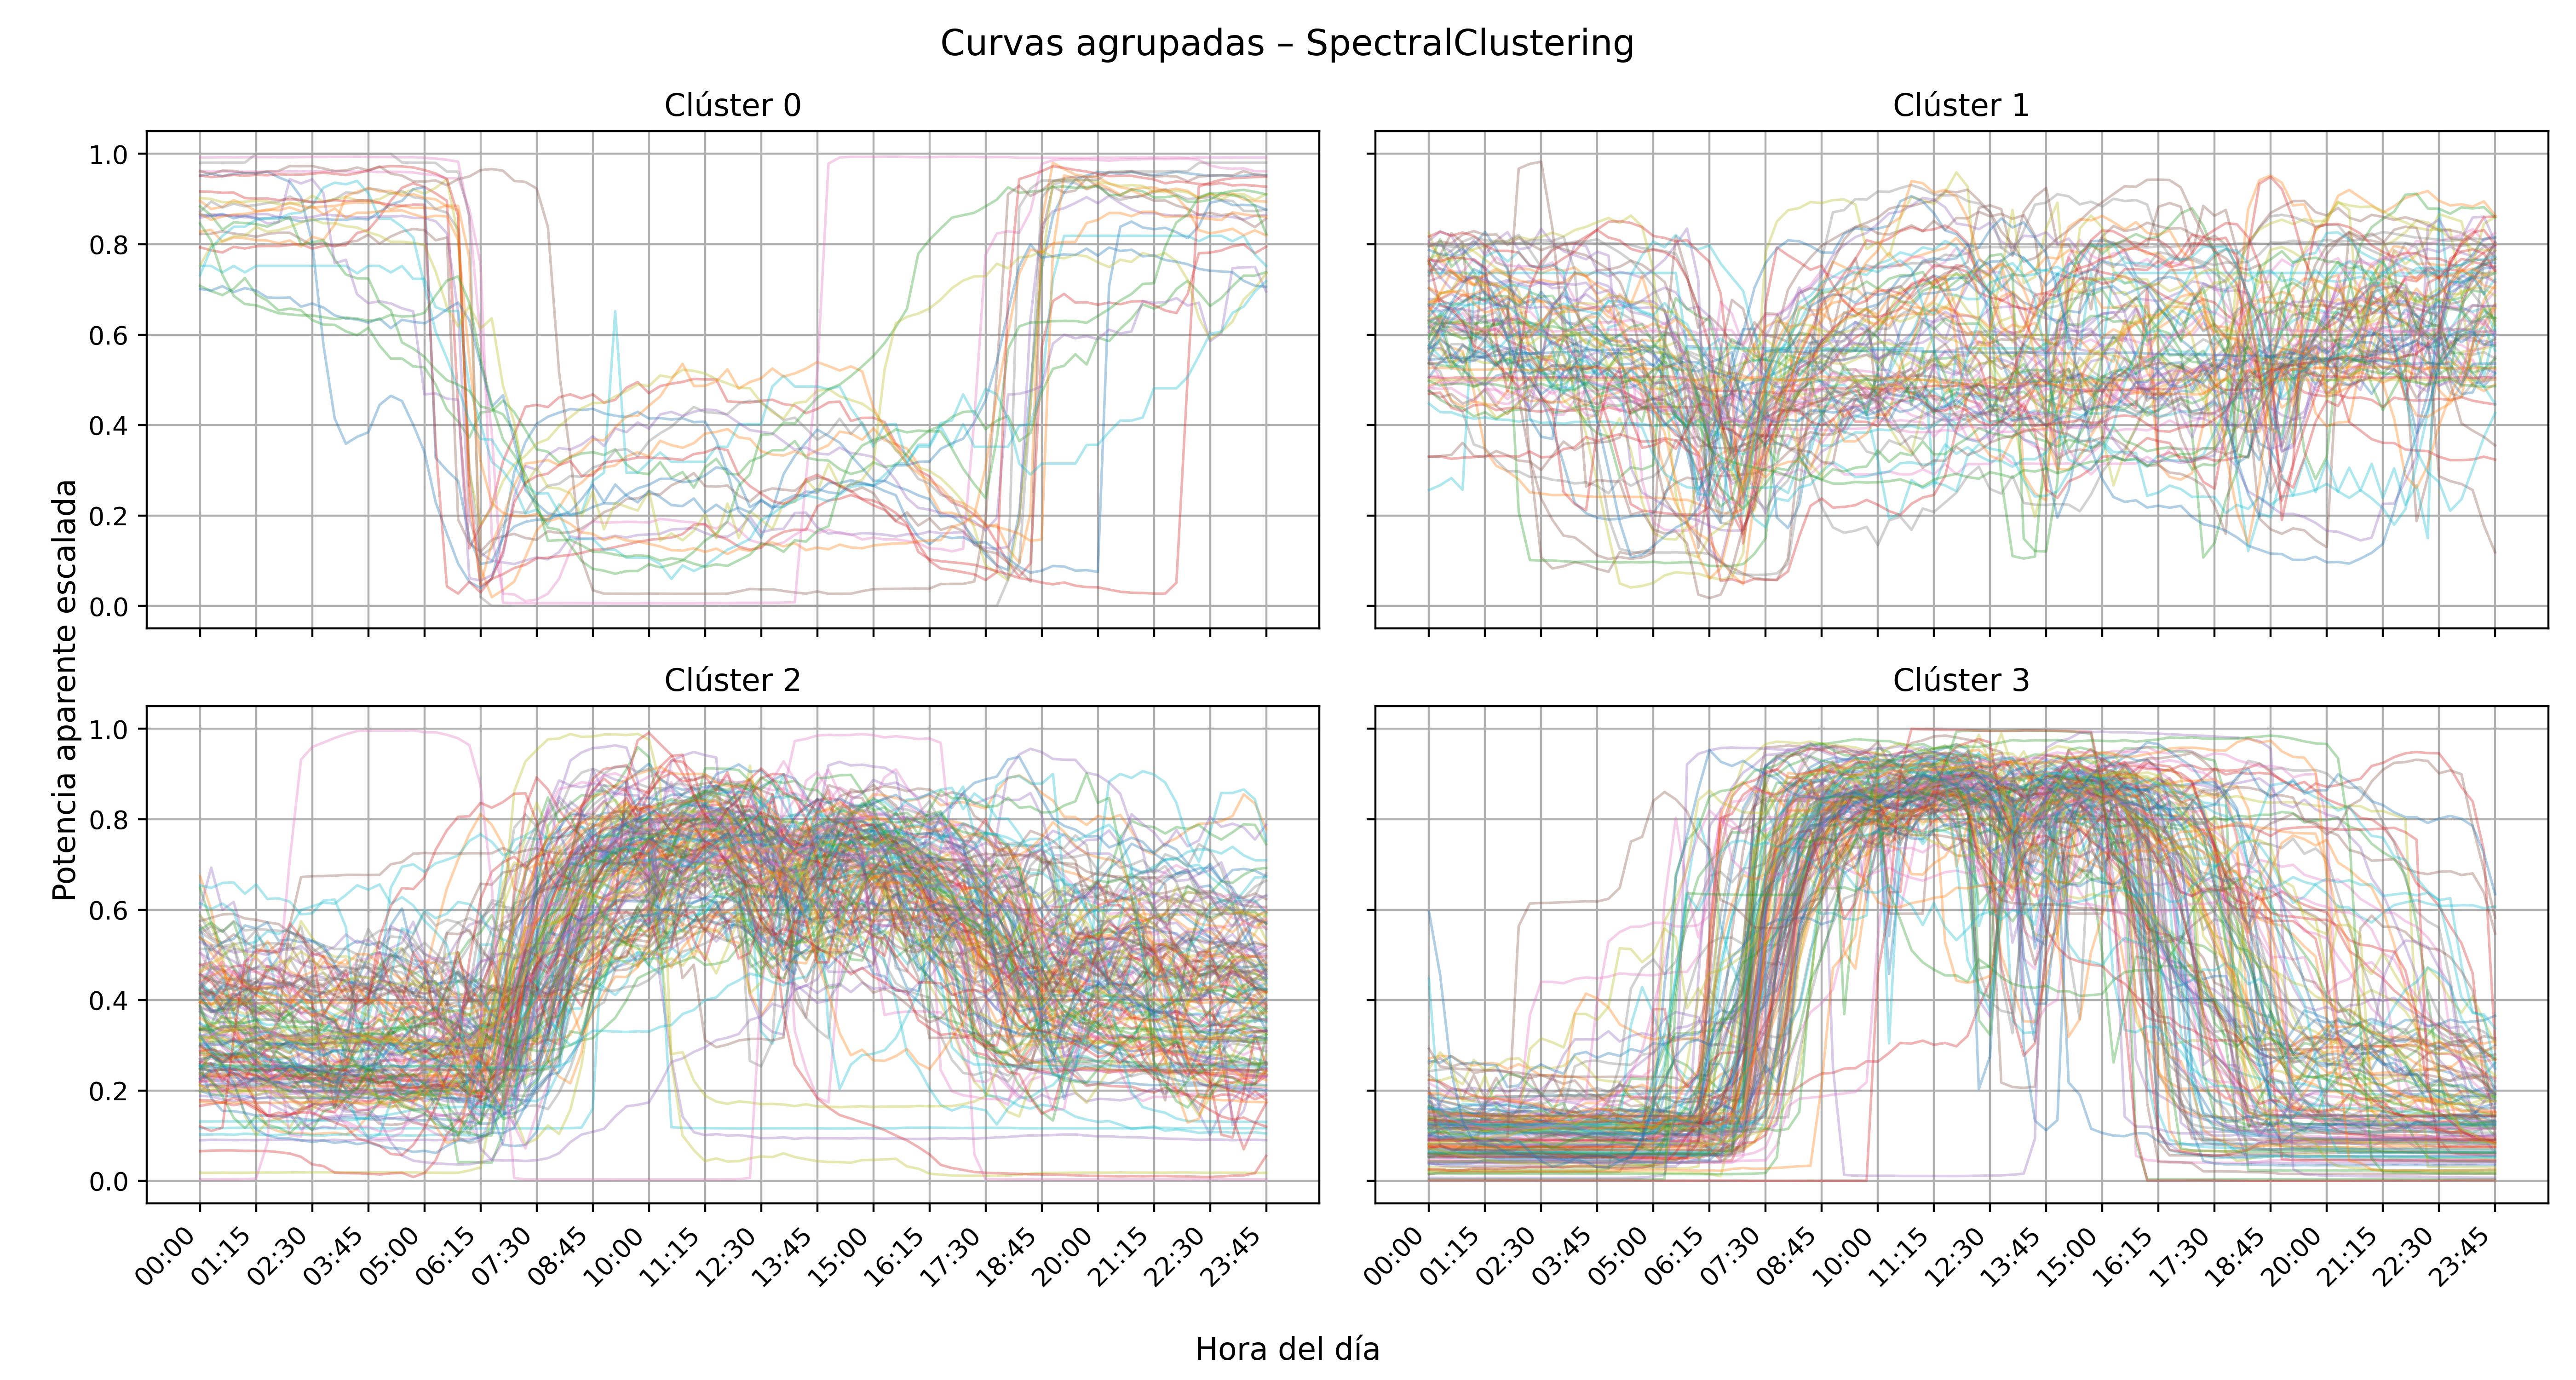
\includegraphics[scale=0.44]{./imgs/curvas_agrupadas_mejor_algoritmo.png}
    \caption{{Spectral Clustering: curvas de carga de los clientes agrupados por clúster.}}
    \label{fig:curvas_clientes_SC}
    \end{center}
\end{figure}


\subsubsection*{Interpretación energética de los clústeres obtenidos}
Al observar las curvas de carga por clúster de manera conjunta, es posible percibir la coherencia interna de los grupos obtenidos y distinguir entre diferentes patrones de consumo. Siguiendo esta observación, a continuación se muestra la interpretación energética de cada clúster que ha sido identificado a través de Spectral Clustering.\\

\begin{itemize}
    \item Clúster 0: Este clúster agrupa aquellos clientes cuyo perfil de consumo muestra niveles altos durante la madrugada, la forma que presentan estas curvas nos indican patrones de funcionamiento que no corresponden a horarios laborables, lo cual indica que estos clientes realizan sus actividades en horarios nocturnos.
    \item Clúster 1: Los clientes agrupados en el presente clúster presentan un comportamiento estable a lo largo del día, sin variaciones claramente definidas. La forma de la curva refleja una dispersión ordinaria, lo cual indica que estos clientes mantienen su actividad sin una estructura horaria dominante.
    \item Clúster 2: Este clúster contiene aquellos clientes cuya forma de curva denota actividad diurna, caracterizada por un incremento sostenido del consumo en horas de la mañana, alcanzando valores elevados durante el día y disminuyendo de manera gradual y progresiva hacia la tarde y noche. Se espera que estos clientes mantengan patrones de consumo concentrados en el período diurno, sin transiciones abruptas entre estados de baja y alta demanda.
    \item Clúster 3: Los clientes pertenecientes a este clúster presentan una forma de curva escalonada, con consumos considerablemente bajos durante la madrugada y un ascenso abrupto en horas de la mañana, una meseta estable durante el día y un descenso igualmente abrupto al finalizar la jornada. Se espera que estos clientes presenten patrones de consumo estructurados y delimitados en intervalos de tiempo claramente definidos.
\end{itemize}

La clara diferenciación entre estos comportamientos confirma que los clústeres obtenidos no solo son estadísticamente consistentes, sino que además presentan una interpretación energética clara y útil, lo cual es fundamental para su aplicación en escenarios reales del sector eléctrico.

\subsection{Selección final del mejor algoritmo}
En base a los resultados cuantitativos (correlación intra-cluster, así como otros factores complementarios) y el análisis cualitativo (curvas tipo y proyección PCA) se escoge el algoritmo Spectral Clustering como el modelo final del componente. Esta elección se produce en base a su mayor correlación intra-cluster media (una valoración que analiza de una manera más directa la similitud estructural de las curvas de carga de cada cluster, en la línea de la finalidad básica del análisis).\\

En consecuencia, el modelo escogido constituye la base para la interpretación de los patrones de consumo eléctrico encontrados en los consumidores no regulados y su posible utilización en los procedimientos de análisis y de planeamiento energético.\\

\section{Conclusiones}
La realización del presente Trabajo de Integración Curricular utilizando algoritmos de aprendizaje no supervisado ha permitido evidenciar que el enfoque de segmentación de clientes en base a la forma de la curva característica anual de consumo constituye un enfoque técnicamente viable y mucho más representativo que los enfoques basados en promedios o en clasificaciones rigidas, al captar la variabilidad y complejidad del patrón real de consumo energético adecuadamente.\\

El uso de la metodología CRISP-DM, adaptada a los objetivos del proyecto, proporcionó un marco de trabajo estructurado y sistemático para comprender el problema, preparar los datos y para poder comparar diferentes algoritmos de clustering de una forma objetiva. La modificación de la fase que proponía seleccionar la mejor agrupación en base a métricas de calidad y homogeneidad se mostraba coherente con la naturaleza exploratoria y no supervisada del análisis.\\

El proceso de extracción, transformación y carga (ETL), implementado a través de Apache Airflow permitio la consolidación de los registros de consumo mensual en curvas anuales representativas normalizadas. Aspectos como la limpieza de datos, interpolación de valores nulos, exclusión de días no laborables y la normalización por día garantizaron consistencia, comparabilidad y la calidad de los datos de entrada para los algoritmos de clustering y posicionó a la fase de preparación de los datos como un aspecto fundamental para asegurar resultados confiables en las etapas posteriores de modelado y evaluación.\\


La implementación y evaluación de los algoritmos K-Means, Gaussian Mixture, Birch y Spectral Clustering demostró que cada una de las técnicas tiene características diferentes en función de la estructura de los datos de consumo. La comparación, mediante las métricas internas de correlación intra-cluster promedio, Silhouette Score, Davies-Bouldin Index y Calinski-Harabasz Index, permitió cuantificar la coherencia interna de las agrupaciones e identificar la mejor separación relativa entre los clústeres.\\

El uso de correlación intra-clúster promedio como principal métrica de evaluación evidenció ser especialmente adecuada para el análisis de las curvas de carga normalizadas, pues ésta permitió cuantificar la similitud en la forma de las curvas de los clientes que componen cada grupo, lo cual se alinea con el objetivo de segmentar a los clientes en función de su patrón característico de consumo y no en función de su magnitud absoluta.\\

La evaluación cualitativa y las visualizaciones complementarias (curvas promedio por algoritmo, curvas individuales y proyección PCA) demostraron que los algoritmos implementados identifican patrones de consumo coherentes y diferenciados, particularmente, la aplicación de la técnica de Análisis de Componentes Principales (PCA), facilitó la interpretación de las agrupaciones obtenidas, dado que permite ofrecer una representación bidimensional de los clústeres para corroborar visualmente la coherencia de los patrones que los algoritmos de clustering han identificado dentro del conjunto de datos.\\

El algoritmo Spectral Clustering, el cual fue seleccionado como el de mejor rendimiento al obtener la mayor correlación intra-cluster promedio, además de proporcionar resultados comparables a los que obtienen los otros algoritmos para las métricas complementarias que fueron utilizadas para evaluarlos, permitió identificar cuatro clústeres con un comportamiento energético claramente diferenciado. Estas agrupaciones permiten evidenciar perfiles de consumo que asociamos a los clientes con una fuerte presencia de actividad nocturna, clientes con una demanda estable durante el día, clientes con un perfil de consumo diurno mayoritario y clientes con un patrón escalonado donde se pueden apreciar ascensos y descensos abruptos de la demanda. Estos hallazgos permiten tener un insumo relevante para el análisis del comportamiento energético de los clientes no regulados, además de aportar información técnica relevante para los procesos de planificación energética y gestión de la demanda.\\

\section{Recomendaciones}
Se recomienda que en futuras aplicaciones operativas del componente se desarrolle un proceso de actualización periódica de las curvas de consumo, para que las segmentaciones recojan cambios en los hábitos de consumo asociados a cambios económicos, productivos o tecnológicos de clientes no regulados.\\

Con el fin de ampliar la caracterización de los segmentos identificados, se recomienda incorporar, en futuros análisis, variables adicionales que no fueron tomadas en cuenta para el presente trabajo, tales como la actividad económica del cliente, datos sobre la climatología e indicadores socioeconómicos. Con este tipo de variables sería posible llegar a explicar de mejor manera los factores que influyen en la identificación de patrones de consumo, así como contribuir en el diseño de estrategias de análisis y gestión. No obstante, esta ampliación puede hacerse sin alterar el enfoque del componente trabajado, el cual se basa únicamente en segmentar a partir de la forma de la curva característica anual de consumo.\\

Se recomienda mantener el uso de métricas orientadas a la similitud estructural de las curvas, como la correlación, en futuros análisis, ya que se demostró su idoneidad frente a índices que tienden a verse dañados por la alta variabilidad inherente a los perfiles de consumo eléctrico.\\

Se propone tomar el componente desarrollado como una base metodológica para futuras tareas de análisis avanzado; por ejemplo, tareas de estudios de proyección de demanda o la identificación de grupos de clientes cuya demanda muestra comportamientos atípicos, aprovechando la infraestructura de datos y el flujo de trabajo ya implementados. En este sentido, podrían explorarse algoritmos de agrupamiento específicos para trabajar con series temporales o técnicas basadas en aprendizaje profundo que permiten captar patrones de variación más complejos en las curvas de carga, sin embargo, cualquier extensión en esta línea de investigación deberá ser evaluada cuidadosamente en función del posible impacto que ello pueda tener en la interpretabilidad de los resultados frente a las técnicas tradicionales así como también justificada con respecto al valor que esta puede aportar.
% REFERENCIAS BIBLIOGRÁFICAS
\chapter{Referencias Bibliográficas}
\printbibliography[heading=none]

\chapter{Anexos}
\section*{Anexo I. Código Python para el DAG de proceso ETL implementado}
El código desarrollado para construir el DAG que compone todo el proceso ETL implementado en Apache Airflow se encuentra disponible en el siguiente enlace: ADJUNTAR ENLACE GITHUB
\section*{Anexo II. Cuaderno de trabajo realizado para la implementación de los modelos de clustering}
La implementación de todos los modelos de clustering mencionados en el presente documento puede encontrarse en un cuaderno de trabajo disponible en el siguiente enlace: ADJUNTAR ENLACE GITHUB

\end{document}
